\documentclass[12pt]{scrartcl}
\usepackage{comment} % enables the use of multi-line comments (\ifx \fi) 
\usepackage[english,german]{babel} 
\usepackage[utf8]{inputenc}
\usepackage{fancyhdr}
\usepackage{graphicx}
\usepackage[article, total={6in, 8in}]{geometry}
\usepackage{float}
\usepackage{wrapfig}
\usepackage[onehalfspacing]{setspace}
\usepackage{url}
\usepackage{tabularx}
\usepackage{pdfpages}
\usepackage{wrapfig}
\usepackage[T1]{fontenc}% wichtig für Trennung von Wörtern mit UmlaPuten
\usepackage{microtype}% verbesserter Randausgleich
\setlength{\headheight}{21.4pt}
\usepackage{apacite}
\usepackage{natbib}
\usepackage{eurosym}
\usepackage{amsmath}
\usepackage{algorithm}
\usepackage{algorithmicx}
\usepackage[noend]{algpseudocode}

\begin{spacing}{1.0}
	\bibliographystyle{apacite}
\end{spacing}
\setlength{\parindent}{0em}
\setlength{\parskip}{2mm}

\makeatletter
\def\BState{\State\hskip-\ALG@thistlm}
\makeatother

\DeclareMathOperator{\EX}{\mathbb{E}}% expected value
\numberwithin{equation}{section}
% Special characters
\usepackage{eucal}
% math alphabet
\usepackage{amssymb}
\usepackage{scrpage2}%
\DeclareMathOperator*{\argmax}{argmax}
\DeclareMathOperator*{\max}{argmax}

%Pseudo-code indent
\algdef{SE}[SUBALG]{Indent}{EndIndent}{}{\algorithmicend\ }%
\algtext*{Indent}
\algtext*{EndIndent}

%%%% footer and header %%%%
\usepackage{scrpage2}%
\pagestyle{scrheadings}%  S
\clearscrheadfoot% 
\setheadwidth{text}%
\automark{section}% 
\ihead{\textbf{\pagemark}}
\renewcommand{\sectionmark}[1]{\markright{\ #1}} 
\ohead{\rightmark}
\setheadsepline{0.5pt}
%%%% \footer and header %%%%

\begin{document}

\begin{titlepage}
	\centering	
	{\scshape\LARGE Hochschule Bremerhaven \par}
	\vspace{1cm}
	{\scshape\Large Exposé für eine Bachelorarbeit zum Thema:\par}
	\vspace{1.5cm}
	{\huge\bfseries Reinforcement Learning\par}
	\vspace{2cm}
	{\Large\itshape Theoretische Grundlagen der tabellarischen Lernmethoden und praktische Umsetzung am Beispiel eines Ameisen-Agentenspiels
	\par}
	\vfill
	\begin{tabularx}{\textwidth}{lX}
		Autor: & Jan Löwenstrom \\
		Matrikelnr.: & 34937 \\
		Erstprüfer: & Prof. Dr.-Ing. Henrik Lipskoch \\
		Zweitprüfer: & Prof. Dr. Mathias Lindemann \\
	\end{tabularx}  
    \vfill

% Bottom of the page with current date
	{\large \today \par}       
\end{titlepage}

% Count title page as first page
\setcounter{page}{2}
\tableofcontents
\pagebreak
\listoffigures
\newpage


\noindent
\section{Einleitung}

Viele Probleme sind derart komplex, besitzen gigantische Zustandsräume oder sind dynamisch, sodass es praktisch unmöglich ist, ein Programm im klassischen Sinne zu entwerfen, das auf jegliche Situation eine vordefinierte beste Lösung hat. In einigen Fällen sind die Anforderungen an den benötigten Speicher oder die Rechenleistung zu enorm, in den meisten Fällen könnten jedoch selbst Menschen aufgrund der gegebenen Faktoren nicht bestimmen, welche die optimale Aktion ist. Es ist somit erstrebenswert, dass ein Computer selber lernt, wie er zu handeln hat und das ausschließlich auf Basis  einer abstrakten Formulierung des eigentlichen Problems und Ziels. \par 
Eine Sammlung von Methoden setzt sich genau mit dieser Thematik auseinander, das Bestärkende Lernen (\textit{Reinforcement Learning}, RL). Neben dem \textit{Supervised Learning} und dem \textit{Unsupervised Learning} ist sie eine der drei Hauptdisziplinen des Maschinellen Lernens.


\subsection{Motivation}
Die Motivation des Autors sich intensiv mit dem Thema Reinforcement Learning auseinanderzusetzen basiert auf drei Gründen.
\par 
Zum einen ist die Arbeit im Zusammenhang mit dem einjährigen Bachelorprojekt zu nennen. In diesem beschäftigte sich eine Gruppe von Studierenden mit dem breiten Thema \glqq Maschinelles Lernen\grqq{}. Neben der Vertiefung in dem Bereich \glqq Neuronale Netze\grqq{} wurde sich auch mit dem sog. \textit{NEAT}-Algorithmus (\textit{NeuroEvolution of Augmented Topologies}) befasst, einem genetischen Algorithmus, der eine Form des Reinforcement Learning darstellt, jedoch nur für Probleme mit kleinem Zustandsraum anwendbar ist \cite[S.~7f]{Sutton1998}.
\par
Ein weiterer Punkt stellt die Belegung eines Wahlpflichtmoduls dar, welches der Autor im Verlauf seines Studiums absolvierte. Dieses Modul trägt den Namen \glqq Agentensysteme\grqq{} und behandelt autark fungierende Softwareagenten, die mit ihrer Umwelt interagieren. Dieses Grundkonzept, dass ein Entscheidungsfinder Aktionen ausführt, um letztendlich ein Ziel zu erreichen, ist annähernd auf das Kontext des Reinforcement Learnings übertragbar. Wohingegen für das Modul auf \glqq klassische\grqq{} Programmierung mit Algorithmen, wie dem \textit{A-Star} oder der Tiefensuche zurückgegriffen wurde, liegt die Motivation für diese Arbeit darin, herauszufinden, ob auch Reinforcement Learning auf die gestellte Semesteraufgabe anwendbar ist.
\par
Komplettiert wird das Ganze dadurch, dass das Thema Reinforcement Learning in den letzten fünf Jahren einen regelrechten Boom erlebt. Untermauert wird diese Behauptung durch die Anzahl der Veröffentlichungen zu diesem Thema in den vergangen Jahren auf dem Dokumentenserver \textit{arXiv.org}. Waren es für das gesamte Jahr 2015 nur 50 Publikationen, so stieg die Zahl der veröffentlichen Papers für das Jahr 2019 auf 1206 \cite[]{arxiv}.


\subsection{Zielsetzung}
Einerseits besteht das Ziel dieser Arbeit darin, einen Überblick über die theoretischen Grundlagen des Reinforcement Learnings, seiner Bestandteile und den tabularen Lernmethoden zu geben. Diese Auseinandersetzung stützt sich vor allem auf die beiden Standardwerke von \cite{Sutton1998} und \cite{Wiering}, sowie der öffentlich zugänglichen Vorlesung der Stanford-Professorin \cite{Brunskill}.
\par
Neben dem theoretischen Teil eine praktische Vertiefung stattfinden. Hierbei soll den Lesenden durch ausführlich beschriebene Zustands- und Belohnungsfunktionsmodellierungen verdeutlicht werden, welche abstrakten Eigenschaften und Voraussetzungen erfüllt sein müssen, um Reinforcement Learning als solches auf eine Problemstellung anwenden zu können.
Des Weiteren sollen Fragen beantwortet werden, die sich darauf beziehen, welchen Einfluss verschiedene Parameter auf den Lernprozess haben und wie sich diese auf das Konvergenzverhalten auswirken.
\par 
Zusätzlich setzt sich der Autor das Ziel, herauszufinden, ob Algorithmen des RLs auf die Semesteraufgabe des Wahlpflichtmoduls \glqq Agentensysteme\grqq{} anwendbar sind und die Fähigkeit beherrschen, implizit Verhalten zu erlenen, welches einem Wegfindungsalgorithmus, wie dem \textit{A-Star}, ähnelt.

\subsection{Struktur der Arbeit}
Die Arbeit besteht aus fünf Teilen. Zu Beginn werden in Kapitel \ref{sec:Grundlagen} die theoretischen Grundlagen hinter dem Reinforcement Learning erläutert. Darauf aufbauend beleuchtet das Kapitel \ref{sec:Lernmethoden} die drei großen Algorithmengruppen. Darunter zählt die Dynamische Programmierung, die Monte-Carlo Methoden und das \textit{Temporal-Difference Learning}. Besonders die letzten beiden Gruppen werden intensiv behandelt, Parallelen zwischen ihnen aufgezeigt und Pseudocode dargestellt.
\par 
Mit dem Kapitel \ref{sec:praktischerTeil} beginnt der praktische Teil der Arbeit, der wiederum in drei Teile gegliedert ist. Zunächst wird die Implementation vorgestellt und spezielle Anforderungen und Herausforderungen während der Erstellung aufgeführt. Anschließend werden zwei Problemszenarien detailliert definiert und beschrieben. Eine ist das episodiale Problem mit dem Namen \textit{Jumping Dino}, das andere ist ein kontinuierliches Problem, welches den Namen \textit{AntGame} trägt.
\par 
Der letzte Teil der Arbeit sind die Ergebniskapitel \ref{sec:ergbJD} und \ref{sec:ergbAG}, in denen u.a. das Konvergenzverhalten und die Auswirkungen bestimmter Lernparameter untersucht werden. Zudem werden theoretische Annahmen mit den praktischen Ergebnissen verglichen, um Schlussfolgerungen zu ziehen.
\par 
Abgeschlossen wird die Arbeit durch ein Fazit und einem Ausblick, welche Problemstellungen oder Methoden beispielsweise bei einer potenziellen Masterarbeit untersucht werden könnten.
\pagebreak

\section{Grundlagen}
	Dieser Teil der Arbeit gibt einen Überblick über sämtliche Bestandteile des Reinforcement Learnings. Dabei wird zunächst der wichtige mathematische Rahmen erläutert, der als Markov-Entscheidungsprozess verstanden wird. Aus diesem Rahmen lässt sich ein generisches Agent-Umwelt-Interface ableiten, auf welches eingegangen wird, um fundamentale Bestandteile, wie Belohnungen, Episoden, Gewinne und Nutzenfunktionen zu erläutern. 
\par
Abgerundet wird der Grundlagenteil mit der Auseinandersetzung von Strategien und dem Streben nach Optimalität, sowie der Darstellung des sog. \textit{Exploration-Exploitation-Dilemmas}.
	\subsection{Markov Entscheidungsprozess}
	\par 
Die Umwelt wird in dieser Arbeit als Markov'scher Entscheidungsprozess (\textit{Markov Decision Process, MDP}) angesehen. Dieses Framework findet häufig Verwendung in der stochastischen Kontrolltheorie \cite[S.~3]{Gosavi} und bietet im Bezug auf das \textit{Reinforcement Learning} Problem den mathematischen Rahmen, um u.a. präzise theoretische Aussagen treffen zu können∏ Als \textit{MDP} versteht sich die Formalisierung von sequentiellen Entscheidungsproblemen, bei denen eine Entscheidung nicht nur die sofortige Belohnung beeinflusst, sondern auch alle Folgezustände und somit auch alle zukünftigen Belohnungen \cite[S.~47]{Sutton1998}. Ein Entscheidungsfinder muss somit das Konzept von verspäteten Belohnungen (\textit{delayed rewards}) durchdringen. Vermeintlich schlecht erscheinende Entscheidungen in der Gegenwart können sich im Nachhinein als optimal herausstellen können, angesichts der gesamten Handlung. Ein Skat-Spieler könnte z.B. alle Trümpfe direkt am Anfang spielen, um einen sofortigen Vorteil zu erhalten. Für den Spielausgang ist es aber womöglich besser, die Trümpfe für einen späteren Zeitpunkt aufzubewahren und zu Beginn \glqq schlechte \grqq{} Entscheidungen zu treffen, die dazu führen, ein paar Stiche zu verlieren.
\par 
Probleme, die als \textit{MDP} definiert werden, müssen die Markov-Eigenschaft erfüllen, da diese gewissermaßen als Erweiterung von Markov-Ketten zu betrachten sind, mit dem Zusatz von Aktionen und Belohnungen. Bei den sog. Markov-Ketten führt das System zufällige Zustandswechsel durch \cite[S.~3]{Gosavi}. Dabei sind die Übergangswahrscheinlichkeiten zu den einzelnen Folgezuständen ausschließlich von dem aktuellen Zustand abhängig und nicht aufgrund des historischen Verlaufs \cite[S.~3]{Gosavi}. Da die Markov-Eigenschaft eine essentielle Voraussetzung bei der Problemmodellierung ist, wird sie in Kapitel X näher erläutert. Die Beziehung zwischen Agent und Umwelt, kann durch folgendes Interface dargestellt werden \cite[S.~48]{Sutton1998}:

\par 

\begin{figure}[H]
    \centering
    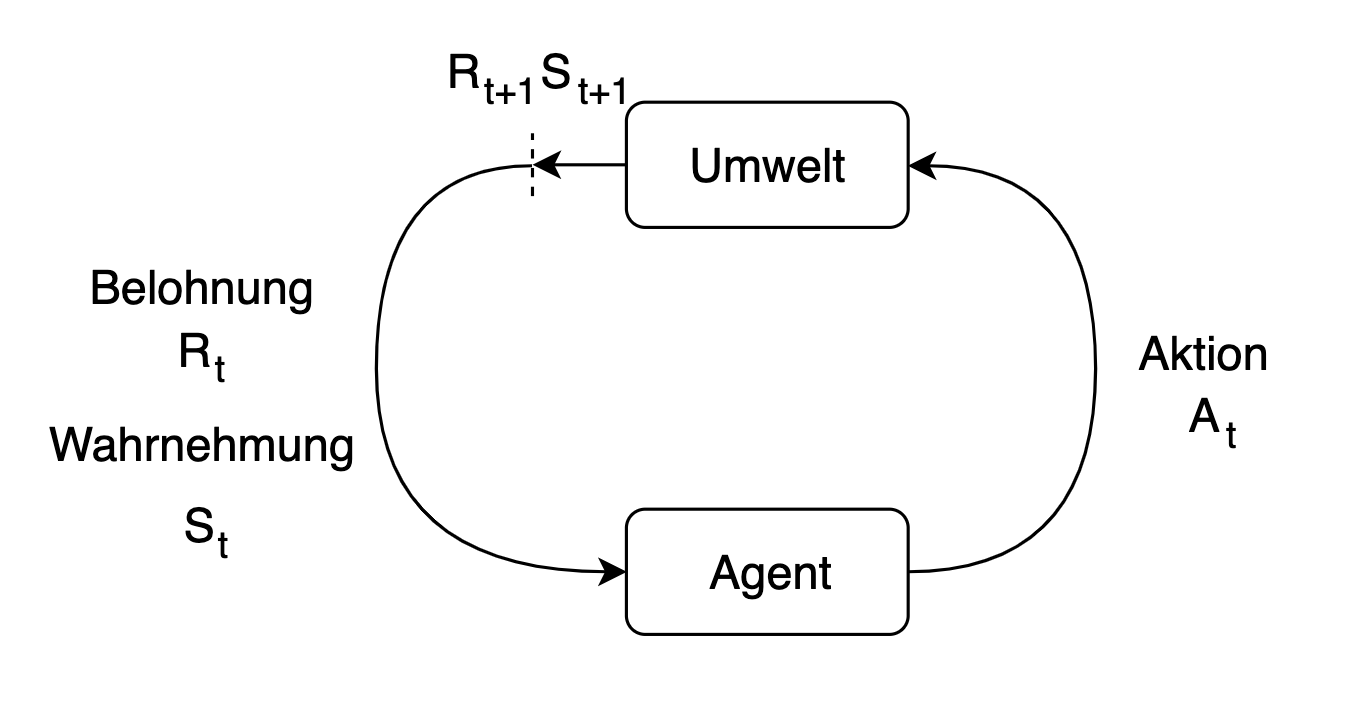
\includegraphics[height=150px]{images/agentUmweltInterface.png}
    \caption{Agent-Umwelt Interface}
\end{figure}


Der Agent interagiert mit dem \textit{MDP} jeweils zu diskreten Zeitpunkten $t = 0, 1, 2, 3, \dots$. \\
Zu jedem Zeitpunkt $t$ beobachtet der Agent den Zustand seiner Umgebung $S_t \in \mathcal{S}$ und wählt aufgrund dessen eine Aktionen $A_t \in \mathcal{A}$. Als Konsequenz seiner Aktion erhält er einen Zeitpunkt später eine Belohnung $R_{t+1} \in \mathcal{R} \subset\mathbb{R} $ und stellt den Folgezustand $S_{t+1}$ fest. 
\par 
In der Literatur findet sich jedoch auch eine abweichende Definition im Bezug auf den Zeitpunkt der Belohnungsvergabe. \cite{watkins1989learning}, \cite{Wiering} und \cite{YuMDP} z.B. binden die Belohnung $R_t$ an das Zustands-Aktions-Paar $(S_t, A_t)$. Die  Definition $R_{t+1}$ bei Aktion $A _{t}$ von \cite{Sutton1998} wird allerdings im Verlauf dieser Arbeit verwendet, da sie besser beschreibt, dass die Belohnung und der Folgezustand gemeinsam berechnet werden und einen Zeitpunkt später, nach Aktion $A_t$, für den Agenten sichtbar sind.
\par 
Das Zusammenspiel zwischen Agenten und MDP erzeugt somit folgende Reihenfolge \cite[~S.48]{Sutton1998}:

\begin{equation}\label{eq:episode}
    S_0, A_0, R_1, S_1, A_1, R_2, S_2, A_2, R_3, \dots
\end{equation}

Wird einfach nur von \textit{MDPs} gesprochen, ist die endliche Variante (\textit{finite MDP}) gemeint, bei dem die Mengen der Zustände, Aktionen und Belohnungen ($\mathcal{S}, \mathcal{A}, \mathcal{R}$) eine endliche Anzahl an Elementen besitzen. In diesem Fall haben die Zufallsvariablen $R_t$ und $S_t$ wohl definierte, diskrete Wahrscheinlichkeitsverteilungen, die nur von dem vorigen Zustand und der vorigen Aktion abhängig sind. Die Wahrscheinlichkeit, dass die bestimmten Werte für diese Variablen $s' \in \mathcal{S}$ und $r \in \mathcal{R}$ eintreten, für einen bestimmten Zeitpunkt $t$ und dem vorigen Zustand $s$ und Aktion $a$, kann somit durch folgende Funktion beschrieben werden \cite[~S.48]{Sutton1998}:

\begin{equation}\label{eq:übergangsfunktion}
p(s',r \mid s,a) \doteq Pr\{S_t=s',R_t=r|S_{t-1}=s,A_{t-1}=a\},
\end{equation}

für alle $s', s \in \mathcal{S}, r \in \mathcal{R}$ und $a \in \mathcal{A}(s)$. Diese Funktion $p$ definiert die sog. Dynamiken (\textit{Dynamics}) eines \textit{MDP}. Sie ist eine gewöhnliche deterministische Funktion mit vier Parametern $p: \mathcal{S} \times \mathcal{R} \times \mathcal{S} \times \mathcal{A} \rightarrow [0,1]$. Das \glqq$\mid$\grqq{} Zeichen kommt ursprünglich aus der Notation für bedingte Wahrscheinlichkeiten, soll hier aber andeuten, dass es sich um eine Wahrscheinlichkeitsverteilung handelt für jeweils alle Kombinationen von $s$ und $a$ \cite[~S.49f]{Sutton1998}:

\begin{equation}\label{eq:wahrscheinlichkeitsverteilung}
\sum_{s' \in \mathcal{S}} \sum_{r \in \mathcal{R}} p(s', r \mid s,a) = 1 \ \forall s \in \mathcal{S}, a \in \mathcal{A}(s)
\end{equation}

Ist das Entscheidungsproblem nicht stochastischer Natur, sondern deterministisch, so ist $p$ immer nur für ein bestimmtes Triplet $(s,a,r)$ für jedes $s' \in \mathcal{S}$ gleich 1, für alle andere jeweils 0. Mit anderen Worten, wird im Zustand $s$ die Aktion $a$ gewählt, führt dies in jedem Fall zu einem bestimmten Folgezustand $s’$. 
\par 

\cite{Sutton1998} erläutern, dass das MDP Framework als extrem flexibel gilt und es demzufolge auf die unterschiedlichsten Probleme angewendet werden kann. Sie führen weiter aus, dass es die nötige Abstraktion für Probleme bietet, bei denen unter Vorgabe eines Ziels mittels Interaktionen gelernt wird. Einzelheiten über das eigentliche Ziel, die Zustände oder die Form des Agenten sind dabei unerheblich. 
Letztendlich kommen die zwei Autoren zu dem Schluss, dass \glqq jedes zielgerichtete Lernen auf drei Signale reduziert werden kann, die zwischen dem Agenten und der Umwelt ausgetauscht werden. Ein Signal repräsentiert die Entscheidung, die der Agent getroffen hat (die Aktion), ein Signal repräsentiert die Basis, auf der er zu dieser Entscheidung gekommen ist (der Zustand) und ein Signal definiert das zu erreichende Ziel (die Belohnung)\grqq{} (S.~50).



	\subsection{Markov-Eigenschaft und Zustandsmodellierung}
	Die Markow-Eigenschaft, obwohl relativ simpel, erhält ein eigenes Kapitel, da sie von fundamentaler Wichtigkeit ist und bei der Modellierung eines Reinforcement Learning Problems eine besondere Rolle spielt. Verbinden lässt sich dies sehr gut mit einem Einblick über die grundsätzliche Modellierung von Zuständen bei einem Reinforcement Learning Problem.

\begin{quote}
    The future is independent of the past given the present
  \end{quote}

Dieser Satz erscheint oft in Büchern und Papern, wenn es um die Markov-Eigenschaft geht, denn er versucht zusammenzufassen, was diese aussagt. Im Zusammenhang von MDPs lässt sich dieser Satz so übersetzen, dass ein Folgezustand nicht abhängig von Aktionen bzw. Zuständen in der Vergangenheit ist, sondern ausschließlich von dem aktuellen Zustand und der aktuell gewählten Aktion.
In der Literatur gibt es unterschiedliche Auffassungen darüber, ob die Markov-Eigenschaft an den MDP direkt geknüpft ist oder an den Zustand, den der Agent zur Abwägung der Entscheidung zur Verfügung hat. Bei der ersten Annahme wird davon ausgegangen, dass der Zustand, der von der Umwelt ausgeliefert wird direkt die Markov-Eigenschaft besitzen muss. (Sutton S.49) hingegen bindet die Eigenschaft an den Zustand und nicht an den Entscheidungsprozess als solches. Ein Zustand ist somit die Menge aller notwendigen Informationen der Vergangenheit, die für die Zukunft relevant sind. Statt den gegebenen Zustand der Umwelt direkt zu übernehmen, werden hier Beobachtungen der Umwelt zu einer internen Repräsentation von Markov-Zuständen verarbeitet.


% \begin{figure}[H]
%     \centering
%     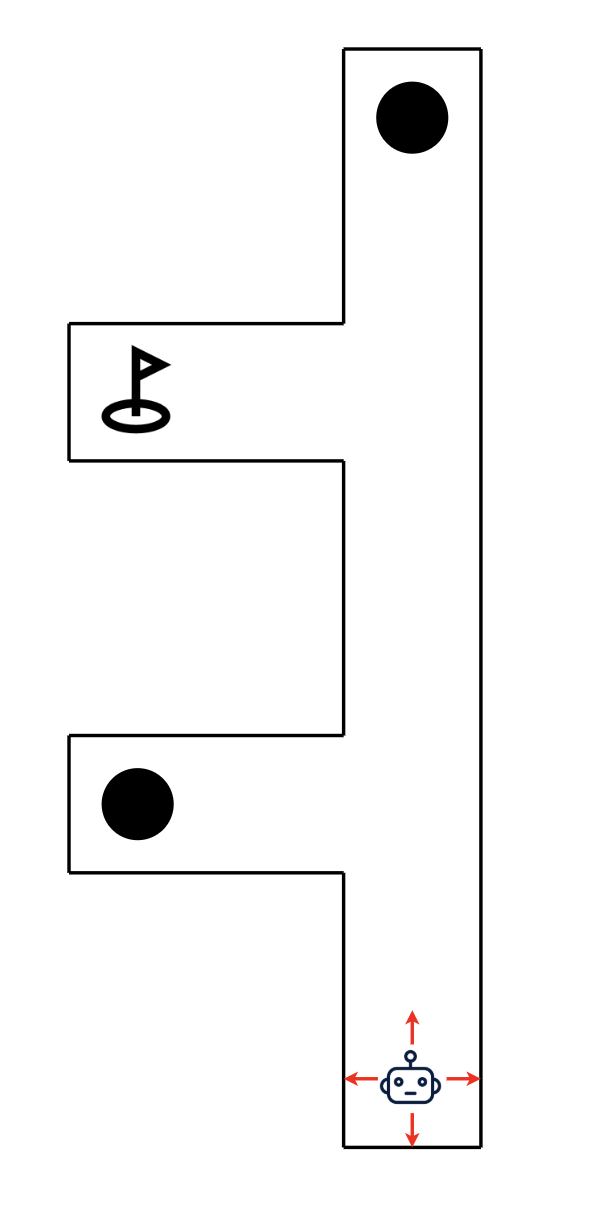
\includegraphics[height=250px]{images/2passagesDefault.png}
%     \caption{ Zwei-Wege Beispiel zu der Markov-Eigenschaft}
% \end{figure}

% \begin{wrapfigure}{L}{0.5\textwidth}
%   \begin{center}
%   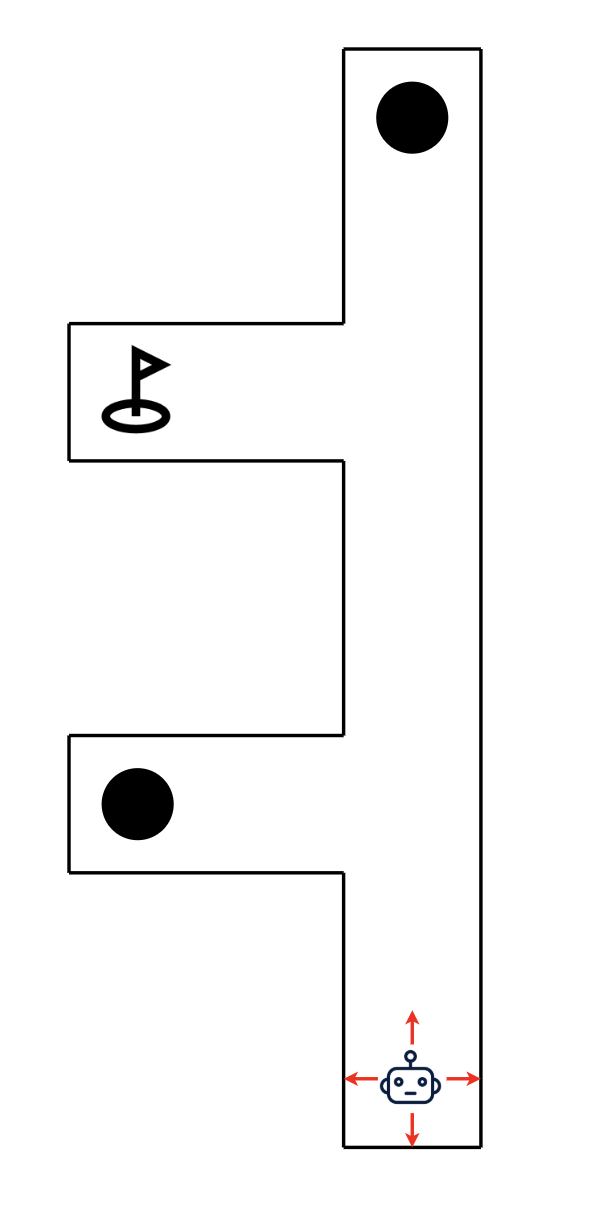
\includegraphics[height=250px]{images/2passagesDefault.png}  \end{center}
%   \caption{Birds}
% \end{wrapfigure}

	\pagebreak

	\subsection{Belohnungen und Zielstrebigkeit}\label{sec:belohnung}
	Das Besondere an dem Reinforcement Learning ist das Belohnungssignal (\textit{Reward}), welches der Agent nach jeder Aktion erhält. Zu jedem diskreten Zeitpunkt wird dem Agenten eine Belohnung in Form einer einfachen Zahl $R_t \in \mathbb{R}$ zugestellt. Aufgabe eines jeden RL-Algorithmus ist es, die Summe aller gesammelten Belohnungen zu maximieren. Dabei ist entscheidend, dass der Fokus nicht ausschließlich auf die sofortigen Belohnungen gerichtet ist, sondern auf die erwartbare Summe aller Belohnungen über einen langen Zeitraum. Entscheidungen, die in der Gegenwart eine hohe sofortige Belohnungen versprechen sind verführerisch, können sich aber in der Zukunft in Bezug auf den gesamten Prozess als suboptimal herausstellen. 
\par 
Eine Belohnungsfunktion wird in der Regeln von einem Menschen definiert und hat den größten Einfluss darauf, wie der Agent sich verhalten soll. Die Festlegung von Belohnung bei bestimmten Events ist die einzige Möglichkeit, die der Agent hat, zu verstehen, welches Ziel er verfolgen soll. Somit ist die Modellierung der passenden Belohnungsfunktion zur korrekten Abbildung der eigentlichen Aufgabenstellung von gravierender Bedeutung.
\par 
Grundsätzlich gibt es zwei Ansätze, um eine Belohnungsfunktion zu formulieren. Verständlich werden diese durch ein Beispiel, bei dem ein Agent lernen soll, Schach zu spielen. Die erste Möglichkeit besteht darin, dem Agenten ausschließlich eine Belohnung aufgrund des Spielausgangs zu geben. Er erhält +1 wenn er gewinnt, -1 bei einer Niederlage und 0 bei Unentschieden (und jeder Aktion zuvor). Auf den ersten Blick erscheint dieser Ansatz trivial, ist aber die direkte Übersetzung des Ziels in eine Belohnungsfunktion. Die größte erwartbare Summe aller Belohnungen erhält der Agent nur, wenn er lernt, das Spiel zu gewinnen. Größter Nachteil dieser Methode ist allerdings, dass der Agent keinerlei Hilfe oder Richtung beim Erkunden des Spiels erhält. Je größer der Zustands- und Aktionraum ist, desto länger braucht er um überhaupt einmal ein Spiel gewinnen zu können und zu lernen, welche Aktionen vorteilhaft sind und welche nicht.
\par 
Um dem entgegenzuwirken, werden dem Agenten bei der zweiten Möglichkeit feingranularere Belohnungen mitgeteilt, statt diese ausschließlich auf das Endresultat zu reduzieren. Bestimmte Belohnungen zeigen dann, ob der Agent seinem Ziel näher gekommen ist oder eine ungünstige Entscheidung getroffen hat. Zum Beispiel könnte dem Agenten eine hohe Belohnung von +10 gegeben werden, wenn er die gegnerische Dame aus dem Spiel nimmt. Es ist auch denkbar, dass jede Spielfeldkonstellation bewertet wird. Dieser Ansatz benötigt somit spezielles Vorwissen über das Problem und kann sich zugleich sehr negativ auf das Verfolgen des eigentlichen Ziels auswirken. Der Agent könnte zum Beispiel nur lernen in jedem Spiel die Dame des Gegners zu schlagen und dabei trotzdem immer die Partie zu verlieren.
\par 
Die korrekte Modellierung der Belohnungsfunktion hat somit eine besondere Bedeutung. Im Beispiel von Schach sollte nur aufgrund des Spielaussgangs bewertet werden. Durchläuft der Agent allerdings ein Labyrinth und soll er so schnell wie möglich hinausfinden, dann sollte nach jeder Aktion eine negative Belohnung von -1 verteilt werden. Somit wird der Agent gezwungen, auf direktem Wege den Zielzustand zu erreichen.
\par 
Prinzipiell gilt: Das Belohnungssignal dient dazu, dem Agenten mitzuteilen \textit{was} er erreichen soll, nicht \textit{wie} er es erreichen soll\cite[S.~54]{Sutton1998}.

	\subsection{Gewinn und Episoden}\label{Gewinne}
	In Kapitel 2.1 wurde gezeigt, dass die Interaktion eines Agenten mit seiner Umwelt als bestimmte Abfolge beschrieben werden kann \eqref{eq:episode}. In ihr werden letztendlich alle Triples von Zustand, ausgeführter Aktion aufgrund dieses Zustands und anschließende Belohnung chronologisch aufgezeichnet. Ist diese Reihenfolge endlich, so wird sie auch als Episode (\textit{Episode}) bezeichnet. Eine Episode fasst somit alle Informationen zusammen, die ein Agent erlebt, während er von einem beliebigen Startzustand aus anfängt die Umwelt zu erkunden. Das Ende einer Episode wird durch das Erreichen eines beliebigen Zielzustands erreicht. Ist eine Episode zu Ende, dann wird das Szenarie zurückgesetzt und der Agent startet erneut im Startzustand. Episoden sind komplett unabhängig voneinander und erzeugen Trajektorien, die nicht von durch vorrige Episoden beeinflusst werden.
\par
Bisher wurde erwähnt, dass das Ziel eines Agenten sei, die Summe der zu erwartenden Belohnungen zu maximieren. Formal betrachtet, versucht er somit die Sequenz der Belohnung, die er nach dem Zeitpunkt $t$ erhält, den sog. erwarteten Gewinn (\textit{Return}), zu maximieren. Im einfachsten Fall sieht $G_t$ wie folgt aus, wobei $T$ der finale Zeitstempel ist.

\begin{equation}\label{eq:simpleReturn}
    G_t = R_{t+1} + R_{t+2} + R_{t+3} + \dots + R_{T}
\end{equation}

Diese simple Addition von nachfolgenden Belohnungen ist ausreichend und sehr praktikabel bei episodialen Problemszenarien. Jedoch ungeeignet für Probleme, bei denen keine klaren Endzustände definiert sind und daher einen sog. unendlichen Horizont (infinite horizon) besitzen. Folglich ist  $T=\infty$, was wiederum bedeutet, dass der Gewinn ebenfalls unendlich ist. 
\par 
Um episodiale und kontinuierliche Aufgaben im Bezug auf den Gewinn zu vereinheitlichen, wird das Konzept der Diskontierung (\textit{discounting}) verwendet. Dabei gibt der Parameter $\gamma$, $0\leq \gamma \leq 1$, Auskunft darüber, wie die Gewichtung zwischen sofortigen und zukünftigen Belohnungen verteilt ist. Der zukünftige diskontierte Gewinn, der durch die Aktion $A_t$ maximiert werden soll, berechnet sich somit wie folgt:

\begin{equation}\label{eq:discountedReturn}
    G_t = R_{t+1} + \gamma R_{t+2} + \gamma^2 R_{t+3} + \dots  = \sum_{k=0}^\infty{\gamma^k R_{t+k+1}}
\end{equation}
Weiterhin ist zu vermerken, dass Gewinne von aufeinanderfolgenden Zeitpunkten miteinander verbunden sind \cite[S.55]{Sutton1998}.

\begin{equation}\label{eq:successiveReturn}
    \begin{aligned}
    G_t &= R_{t+1} + \gamma R_{t+2} + \gamma^2 R_{t+3} + \gamma^3 R_{t+4} + \dots \\
    &= R_{t+1} + \gamma (R_{t+2} + \gamma R_{t+3} + \gamma^2 R_{t+4} + \dots)  \\
   & = R_{t+1} + \gamma G_{t+1}
    \end{aligned}
\end{equation}
Ist $\gamma = 0$, dann wählt der Agent seine Aktionen ausschließlich aufgrund der sofortigen Belohnung. Je näher $\gamma$ an 1 ist, desto "weitsichtiger" wird der Agent, da der Gewinn für den Zeitpunkt $t$ sich zusätzlich aus zukünftigen Belohnungen zusammensetzt. Bei Problemen, die sich in Episoden unterteilen lassen, ist es üblich, dass $\gamma = 1$ ist, sodass der Agent seine Entscheidungen immer aufgrund jeglicher Konsequenzen in der Zukunft bzw. bis zum Ende der jeweiligen Episode trifft. Um zu erreichen, dass die unendliche Summe in \eqref{eq:discountedReturn} bei kontinuierlichen Aufgaben einen endlichen Wert annimmt, muss $\gamma < 1$ \cite[S.55]{Sutton1998}. 
\par 
Probleme mit unendlichen Horizont können durch die Vergabe einer künstlichen Schranke zu einer episodialen Aufgabe umformuliert werden. Denkbar z.B. durch die Festlegung der maximalen Anzahl an Aktionen oder besuchten Zustände. 
\par 
Die Algorithmen der Monte-Carlo-Methoden, die in Kapitel X vorgestellt werden, können ausschließlich auf Basis von Episoden lernen. Jedoch existieren auch Methoden, wie das Temporal-Difference-Learning (Kapitel X), die neben dem episodialen Lernen, zusätzlich in der Lage sind, mit kontinuierlichen Aufgaben zurechtzukommen. 

	\subsection{Strategie und Nutzenfunktion}
	Fast alle Lernalgorithmen des Reinforcement Learning versuchen eine sog. Nutzenfunktion (\textit{Value Function}) zu schätzen. Diese Funktion sagt aus, \glqq wie gut\grqq{} es ist, dass sich der Agent in einem bestimmten Zustand befindet oder eine bestimmte Aktion in einem Zustand ausführt. Dabei bezieht sich das \glqq wie gut\grqq{} darauf,
welche Belohnungen in der Zukunft erwartbar sind, dementsprechend wie groß der erwartete Gewinn ist. Zukünftige Belohnungen sind natürlicherweise abhängig davon, wie sich der Agent verhalten oder vielmehr welche Entscheidungen er in der Zukunft treffen wird. Nutzenfunktion sind deshalb immer in Bezug auf eine bestimmte Strategie definiert \cite[S.~58]{Sutton1998}.
\par 
Eine Strategie (\textit{Policy}) kann als Abbildung verstanden werden, die jedem Zustand eine diskrete Wahrscheinlichkeitsverteilung über Aktionen zuordnet. Folgt der Agent einer Strategie $\pi$ zum Zeitpunkt $t$, dann gibt $\pi(a\mid s)$ an, mit welcher Wahrscheinlichkeit $A_t = a$ ausgeführt wird, wenn $S_t = s$ \cite[S.~58]{Sutton1998}. Neben solchen stochastischen Strategien, existieren auch simplere, deterministische Strategien, die jedem Zustand nur genau eine Aktion zuordnen, $\pi (s) = a$ \cite[]{Brunskill}.
\par
Wie anfangs erwähnt, gibt es zwei Varianten der Nutzenfunktion. Die erste sagt aus, wie groß der Erwartungswert des Gewinns für den Zustand $s$ ist, wenn in diesem gestartet und anschließend aufgrund der Strategie $\pi$ gehandelt wird. Dieser \textit{Zustands-Nutzen} kann für alle $s \in \mathcal{S}$ folgendermaßen definiert werden \cite[S.~58]{Sutton1998}:
\begin{equation}\label{eq:valueFunction}
    v_\pi(s) = \EX_\pi[G_t \mid S_t = s] = \EX_\pi \left[\sum_{k=0}^\infty{\gamma^k R_{t+k+1} \mid S_t = s} \right]
\end{equation}

Die zweite Variante gibt Auskunft darüber, wie groß der Nutzen ist, wenn im Zustand $s$ gestartet, daraufhin die Aktion $a$ ausgeführt und anschließend der Strategie $\pi$ gefolgt wird. $q_\pi$ wird auch als \textit{Aktions-Nutzenfunktion} für die Strategie $\pi$ bezeichnet und wird formal ausgedrückt durch \cite[S.~58]{Sutton1998}:
\begin{equation}\label{eq:actionValueFunction}
    q_\pi(s,a) = \EX_\pi[G_t \mid S_t = s, A_t = a] = \EX_\pi\left[\sum_{k=0}^\infty{\gamma^k R_{t+k+1} \mid S_t = s, A_t = a}\right]
\end{equation}

//TODO der Erwartungswert auf ?
//TODO funktionsapproximation hier? 

	\subsection{Optimalität} \label{sec:optimality}
	Ein Reinforcement Learning Problem zu lösen bedeutet, eine Strategie zu finden, die den größten Gewinn bringt. Dabei lassen sich Strategien vergleichen, insofern, dass eine Strategie besser als eine andere ist, wenn der erwartete Gewinn für alle Zustände größer oder gleich ist \cite[S.~62f]{Sutton1998}. Mit anderen Worten, $\pi \geq \pi'$ gilt, wenn $v_\pi(s) \geq v_{\pi'}(s)$ für alle $s \in \mathcal{S}$. Es existiert mindestens eine Strategie, die besser oder gleich gegenüber allen anderen Strategien ist. Diese ist die optimale Strategie $\pi_*$. \newpage
Optimale Strategien teilen dieselbe (optimale) Zustands-Nutzenfunktion $v_*$ und (optimale) Aktions-Zustands-Nutzenfunktion $q_*$ \cite[S.~62f]{Sutton1998}:

\begin{equation}\label{eq:optimaleValueFunction}
    v_*(s) = \max_\pi v_\pi(s)
\end{equation}
\begin{equation}\label{eq:optimaleActionValueFunction}
    q_*(s,a) = \max_\pi q_\pi(s,a)
\end{equation}

Nutzenfunktionen sind, wie im vorigen Kapitel erläutert, immer abhängig von einer bestimmten Strategie, da diese die gesammelte Erfahrung und somit gleichermaßen die erwarteten, geschätzten Gewinne beeinflusst. Die optimale Nutzenfunktion kann jedoch auch ohne Referenz auf eine konkrete Strategie beschrieben werden, da der Gewinn eines Zustands unter einer optimalen Strategie gleich dem erwarteten Gewinn für die beste Aktion in diesem Zustand ist. $v_*(s)$ referenziert somit $v_*(s')$, den besten Folgezustand, wodurch eine rekursive Beziehung zustande kommt. Eine optimale Nutzenfunktion $v_*$ kann formal folgendermaßen beschrieben werden \cite[S.~63]{Sutton1998}:

\begin{equation}\label{eq:bellmanValue}
    \begin{aligned}
        v_*(s) &= \max_a \EX_{\pi_*}[G_t | S_t = s, A_t = a] \\
        &= \max_a \EX{\pi_*}[ R_{t+1} + \gamma G_{t+1} | S_t = s, A_t = a] \\
        &= \max_a \EX[ R_{t+1} + \gamma v_*(S_{t+1}) | S_t = s, A_t = a] \\
        &= \max_a \sum_{s',r}p(s', r | s,a)[r+ \gamma v_*(s')]
    \end{aligned}
\end{equation}

Diese Gleichung ist die sog. \textit{Bellman Optimality Equation} und lässt sich auch als Gleichungssystem interpretieren, welches eine Gleichung pro Zustand besitzt. Für ein Problem mit $n$ Zuständen ergeben sich somit $n$ Gleichung mit $n$ Unbekannten \cite[S.~63]{Sutton1998}. Eine Berechnung der optimalen Nutzenfunktion ist folglich in der Theorie möglich, jedoch muss die Übergangsfunktion $p$ bekannt sein. Ist $p$ gegeben, wird von einem perfekten Modell gesprochen, eine Voraussetzung, die nicht immer erfüllt ist.
\par 
Selbst wenn die Dynamiken der Umwelt bekannt sind, kann die benötigte Rechenzeit zur Lösung jedoch utopische Ausmaße annehmen. Bei einem Spiel wie \glqq Backgammon\grqq{} sind die Regeln klar definiert, ein perfektes Modell ist demzufolge vorhanden, aber es existieren $10^{23}$ Zustände, was die mathematische Berechnung von $v_*$ mit der \textit{Bellman Optimality Equation} praktisch unmöglich macht \cite[S.~66]{Sutton1998}. Dennoch stellt sie ein wichtiges Fundament für das Reinforcement Learning dar, da die meisten Reinforcement Learning Algorithmen als annäherungsweises Lösungsverfahren verstanden werden können \cite[S.~66]{Sutton1998}. 
\newpage
Methoden des Reinforcement Learnings, die die Umwelt als Blackbox betrachten, werden auch als \textit{model-free} beschrieben. Sie benötigen keinen Zugriff auf die Übergangsfunktion $p$, denn es wird ausschließlich aufgrund der erhaltenen Belohnungen und Beobachtungen gelernt. Hierbei bezieht sich der Lernprozess darauf, wie nah die geschätzte Nutzenfunktion der aktuellen Strategie $\pi$ an $v_*$ bzw. $q_*$ ist.
\par 
Die optimale Strategie lässt sich leicht ermitteln, wenn eine optimale Nutzenfunktion gegeben ist. Ist zum Beispiel $v_*$ vorhanden und befindet sich der Agent in Zustand $s$, dann muss er eine Aktion vorausschauen, um den Folgezustand $s'$ zu finden, der den maximalen Nutzen hat. Dieses Voraussehen benötigt jedoch ein perfektes Modell der Umgebung, um die Übergänge für jede Aktion zu berechnen. Das ist der ausschlaggebende Grund, warum bei \textit{model-free} Methoden $q_*$ berechnet wird. Denn dieser Nutzen umfasst implizit den Nutzen der Folgezustände für jede Aktion. Infolgedessen muss der Agent im Zustand $s$ nur evaluieren, welche Aktion $a$ und somit welches Zustands-Aktions-Paar den größten Nutzen hat und wählt genau jene Aktion.
\par 

\par 

	\subsection{Generalized Policy Iteration}\label{sec:GPI}
	Bei der Berechnung einer optimalen Strategie $\pi_*$ spielt ein zugrundeliegendes Konzept  bei jeglichen Lernmethoden eine wichtige Rolle, die sog. \textit{Generalized Policy Iteration (GPI)}. Dieses, durch \cite{Sutton1998} geprägte, Prinzip beschreibt die Interaktion von zwei nebenläufigen Prozessen (S.~86). Ein Prozess sorgt dafür, dass die Nutzenfunktion beständig für die aktuelle Strategie wird. Er versucht das sog. \textit{Prediction Problem} zu lösen, bei dem die Nutzenfunktion $v_{\pi}$ oder $q_{\pi}$ geschätzt werden muss. Jener Prozess wird als \textit{Policy Evaluation} bezeichnet und unterscheidet sich je nach verwendeten Lernverfahren. \textit{Model-based} Lernmethoden, bei denen ein perfektes Modell vorhanden ist, können den Nutzen für eine Strategie entweder direkt oder iterativ berechnen. Hingegen benötigt die große Gruppe der \textit{model-free} Methoden die gesammelte Erfahrung durch eine Interaktion mit der Umwelt. Hierbei konvergiert der geschätzte Gewinn zu dem tatsächlichen Gewinn, solange jedes Zustands-Aktions-Paar unendlich oft besucht wird. Die Konvergenz lässt sich durch das \glqq Gesetz der großen Zahlen\grqq{} (\textit{Law of large numbers}) begründen.
Ebendies sagt aus, dass die relative Häufigkeit eines Zufallsergebnisses bei zunehmender Anzahl der Ausführungen gegen die theoretische Wahrscheinlichkeit konvergiert. Für einen kompletten mathematischen Beweis siehe \cite[S.~181-189]{dekking2006modern}.
\par 
Das Wissen über den Nutzen der aktuellen Strategie $\pi$ wird von dem zweiten Prozess genutzt, um eine verbesserte Strategie $\pi'$ zu finden. Folgerichtig wird dieser Prozess als \textit{Policy Improvement} betitelt, der das sog. \textit{Control Problem} zu lösen versucht.
\par 
GPI an sich beschreibt lediglich, dass diese zwei Prozesse miteinander Interagieren. Dabei konkurrieren sie auf der einen Seite, weil sie in unterschiedliche Richtungen ziehen. Eine Verbesserung der Strategie bei dem \textit{Policy Improvement}, indem die Strategie gierig im Bezug auf die Nutzenfunktion gemacht wird, führt dazu, dass die evaluierte Nutzenfunktion für die verbesserte Strategie inkorrekt wird \cite[S.~86]{Sutton1998}. Die erneute Evaluierung der Nutzenfunktion bei der \textit{Policy Evaluation} sorgt indirekt dafür, dass die Strategie nicht mehr gierig ist \cite[S.~86]{Sutton1998}.
\par 
\begin{figure}[H]
    \centering
    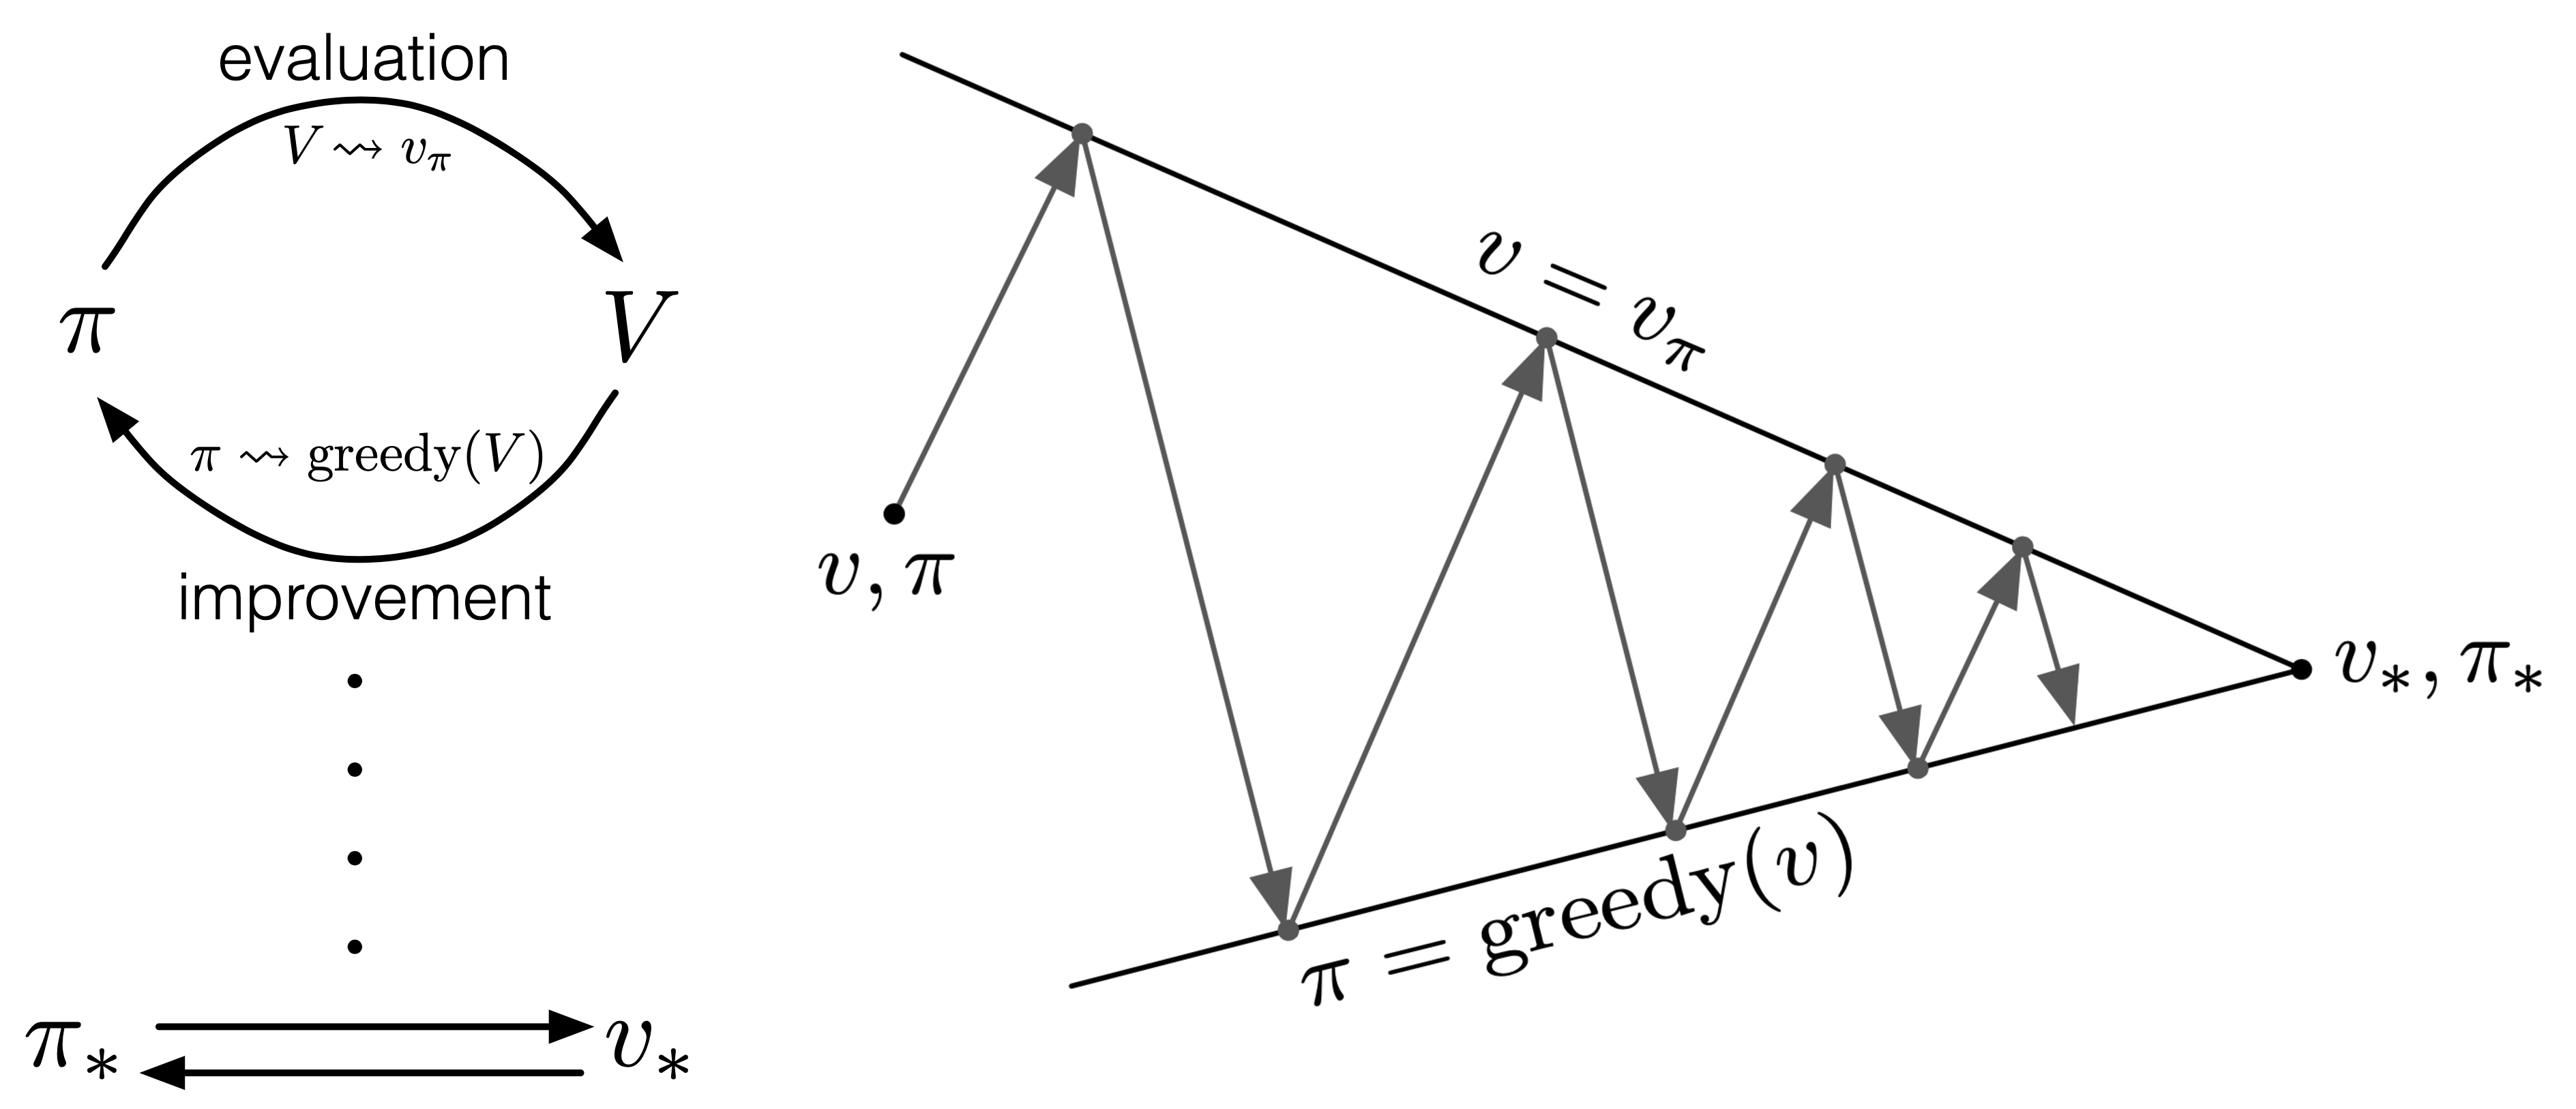
\includegraphics[width=0.7\textwidth]{images/gpi.jpg}
    \caption{GPI nach \cite[S.~86f]{Sutton1998}}
    \label{fig:GPI}
\end{figure}

Auf der anderen Seite kooperieren sich jedoch in dem Sinne, dass beide Prozesse sich nur dann Stabilisieren, wenn eine Strategie durch eine eigens evaluierte Nutzenfunktion gefunden worden ist, die zugleich gierig im Bezug auf genau diese ist, siehe Abb. \ref{fig:GPI}. Sie haben somit ein gemeinsames Ziel, die optimale Nutzenfunktion und die optimale Strategie zu finden.

	\subsection{Exploration-Exploitation Dilemma}
	Durch die Vergabe von Belohnungen und dem übergeordnetem Ziel eines Agenten so viele Belohnungen wie möglich zu sammlen, ergibt sich eine spezielle Problematik bei dem Reinforcement Learning, die bei anderen Lernmethoden des Maschinellen Lernens nicht vorhanden ist. Um den Gewinn zu maximieren, muss der Agent auf der einen Seite Aktionen bevorzugen, die sich in der Vergangenheit bereits als gut herausgestellt haben. Er nutzt unvollständige Erfahrung, um so ausbeuterisch wie möglich zu handeln (\textit{Exploitation}). Andererseits ist der Agent dazu gezwungen, neue Aktionen auszuprobieren, damit der Zustands- und Belohungsraum weiter erkundet wird, um bessere oder sogar optimale Entscheidungen in der Zukunft treffen zu können (\textit{Exploration}). 
\par 
Das Dilemma besteht darin, dass weder Exploration noch Exploitation ausschließlich verfolgt werden kann ohne dabei die eigentliche Lernaufgaben zum Scheitern zu bringen. Dieses Exploration-Exploitation Dilemma wird von Mathematikern seit Jahrzehnten intensiv untersucht, bleibt allerdings ungelöst. Grundsätzlich muss ein Entscheidungsfinder  eine Reihe von unterschiedlichen Aktionen ausführen und zunehmend jene bevorzugen, die sich als gut herausstellen. Dementsprechend muss eine Balance zwischen den beiden Prozessen gefunden werden. \cite[S.~3]{Sutton1998}.
Eine Strategie, die ausschließlich ausbeuterisch handeln, wird auch als gierig (\textit{greedy}) bezeichnet. Der Begriff "gierig" bezeichnet in der Informatik eine Vorgehenweise, bei der immer die, zum Zeitpunkt der Wahl, vermeintlich beste Entscheidungen getroffen wird. Dabei wird die Suche nach einem globalen Maximum komplett untergraben \cite[S.~203]{greedy}. Auf den Kontext des Reinforcement Learning übertragen, wählt eine gierige Strategie für jeden Zustand immer jene Aktion, die den derzeitigen größten Nutzen besitzt. Nur wenn die Nutzenfunktion zu einer optimalen Nutzenfunktion konvergiert ist, ist eine gierige Nutzenfunktion auch gleichzeitig die optimale Strategie. Um jedoch die optimale Nutzenfunktion zu finden, muss erkundet werden.
\par
Ein trivialer, aber denoch effektiver Ansatz ist es, die meiste Zeit gierig zu handeln, aber mit einer geringen Wahrscheinlichkeit $\epsilon$ eine zufällige Aktion auszuführen. Dabei spielen die geschätzen Nutzen der Aktionen keine Rolle und jede Aktion hat die gleiche Wahrscheinlichkeit ausgewählt zu werden. Solche Strategien werden dementsprechend als $\epsilon-greedy$ bezeichnet. \cite[S.~28]{Sutton1998}. Zu vermerken ist, dass die gierige Aktion $A_*$ ebenfalls in der Menge $\mathcal{A}(S_t)$ enthalten ist.

\begin{equation}\label{eq:greedyProbs}
    \pi(a|S_t) =   
        \begin{cases}
            1-\epsilon + \epsilon / |\mathcal{A}(S_t)|      & \quad \text{wenn } a = A_* \\
            \epsilon / |\mathcal{A}(S_t)|  & \quad \text{wenn } a \neq A_*
        \end{cases}
\end{equation}

	\subsection{Zusammenfasung}
	Das Reinforcement Learning wird duch den theoretischen Rahmen der \textit{Markov-Entscheidungsprozesse} beschrieben. Dabei interagiert ein Softwareagent zu diskreten Zeitstempeln mit seiner Umgebung. Als Reaktion auf seine gewählte \textit{Aktion} $a$ zum Zeitpunkt $t$ erhält er einen Zeitpunkt später eine \textit{Belohnung} $r$ und den veränderten \textit{Zustand} $s$ der \textit{Umgebung}.
\par 
Wird die Interaktion durch einen Terminalzustand beendet, so handelt es sich um ein Problem, welches \textit{Episoden} erzeugt. Existiert kein Terminalzustand und somit ein unendlicher Zeithorizont, dann ist dies ein \textit{kontinuierliches} Problem.
\par 
Das Ziel eines jeden RL-Algorithmus ist es, die Summe aller erhaltenen Belohnungen, den sog. \textit{Gewinn}, auf lange Sicht zu maximieren. Für episodale Probleme wird der Gewinn durch die Summe aller erhaltenen Belohnungen pro Episode gebildet. Bei kontinuierlichen Problemen ist dies jedoch nicht möglich, da diese Summe unendlich ist. Aus diesem Grund wird der \textit{Diskontierungsfaktor} $\gamma$ eingeführt. Je kleiner $\gamma$ gewählt ist, desto \glqq kurzsichtiger\grqq{} wird der Agent, da Belohnungen der Zukunft nicht mehr Teil des Gewinns sind.
\par 
Um optimales Verhalten zu erreichen, spielen vor allem zwei Konstukte eine Rolle. Zum einen der sog. \textit{Nutzen}, der aussagt, wie \glqq gut\grqq{} ein Zustand $q(a)$ oder ein Zustands-Aktions-Paar $q(s,a)$ ist. \glqq Nutzen\grqq{} ist eine Schätzung über die tatsächliche, erwartbare Summe aller Belohnungen, die der Agent erhählt, nachdem er sich in einem bestimmten Zustand befindet oder eine bestimmte Aktion in einem Zustand ausgeführt hat. Bei den tabularen Lernmethoden werden alle Werte der Nutzen in einer \glqq Tabelle\grqq{} (oder \textit{Map}) gespeichert, wodurch der Name zustande kommt.  
Zum anderen die \textit{Strategie} $\pi$, die Zustände auf Aktionen mappt und die Entscheidungen bzw. das Verhalten des Agenten steuert. In dieser Arbeit wird hauptsächlich eine $\epsilon$\textit{-greedy} Strategie verwendet, die mit einer Wahrscheinlichkeit von $\epsilon$ eine zufällige Aktion auswählt und mit einer Wahrscheinlichkeit von $1-\epsilon / |\mathcal{A}|$ jene Aktion, die aktuell den höchsten Nutzen besitzt. Diese $\epsilon$\textit{-greedy} Strategie ist zudem ein Lösungsansatz zur Vermeidung des sog. \textit{Exploration-Exploitation-Dilemmas}, da sie sowohl den Zustands- und Aktionsraum erkundet, als auch gierig handelt, um den größten Gewinn zu erhalten.
\par 
Eines der wichtigsten Konzepte, wenn es um Markov-Entscheidungsprozesse und der Modellierung der Zustände für das Reinforcement Learning geht, ist die sog. Markov-Eigenschaft. Diese sagt aus, dass ein Folgezustand nicht abhängig von Aktionen und Zuständen in der Vergangenheit ist, sondern ausschließlich von dem aktuellen Zustand und der aktuell gewählten Aktion. Ein Zustand muss folgerichtig alle nötigen Informationen der Vergangenheit beinhalten, die notwendig sind, um eine optimale Entscheidung treffen zu müssen.

\section{Lernmethoden}
	\subsection{Dynamische Programmierung}
	Die Algorithmen der Dynamischen Programmierung (\textit{Dynamic Programming}, DP) sind im Rahmen dieser Arbeit nicht implementiert und weiter untersucht worden. Dennoch ist ein grundlegendes Verständnis für die DP von Vorteil, da elementare Bestandteile auch in den nachfolgenden Kapiteln zu den Monte-Carlo Methoden (\ref{sec:MC}) und dem \textit{Temporal-Difference Learning} (\ref{sec:TD}) referenziert werden und als Grundlage für das, in Kapitel \ref{sec:GPI} beschriebene, Konzept der \textit{Generalized Policy Iteration} dienen.
\par 
Die grundlegende Idee der Dynamischen Programmierung ist die Aufteilung eines Optimierungsproblems in Teilprobleme. Dabei wird mit einem trivialem Problem gestartet und die optimale Lösung für jenes in einer Tabelle gespeichert, welches anschließend für die Lösung eines sukzessiv größer werdenden Problems verwendet wird \cite[S.~243]{mehlhorn}.
\par 
Bezogen auf das Reinforcement Learning, ist dieses Problem die Suche nach der optimalen Strategie $\pi_*$ genauer gesagt der Lösung der \textit{Bellman Optimality Equation}, siehe \ref{eq:bellmanValue}. Wie bereits in Kapitel \ref{sec:optimality} erwähnt, ist es möglich dieses Gleichungssystem zu lösen und somit $v_*$ oder $q_*$ linear zu berechnen. Mithilfe der DP erschließt sich jedoch ein iterativer Weg.
\par 
Da die Algorithmen der Dynamischen Programmierung Zugriff auf die Übergangswahrscheinlichkeiten der Umwelt sowie der Belohnungsfunktion haben müssen, ist ein perfektes Modell der Umgebung Voraussetzung. DP-Methoden sind folgerichtig immer \textit{model-based}.
\par

\subsubsection{Strategieevaluierung}\label{sec:evaluierung}
Wichtiger Bestandteil eines jeden RL Algorithmus ist die Berechnung der Zustands-Nutzenfunktion $v_\pi$ (oder Aktions-Nutzenfunktion $q_\pi$) für eine willkürliche Strategie $\pi$. Die geschätzte Nutzenfunktion (unter einer bestimmten Strategie) gegen die wahren erwartbaren Werte der Gewinne streben zu lassen, wird auch als Strategieevaluierung (\textit{Policy Evaluation}) bezeichnet \cite[S.~74]{Sutton1998}.
\par 
Die Vorgehensweise der DP um dieses Vorhersageproblem (\textit{Prediction Problem}) zu lösen, lässt sich folgendermaßen beschreiben. Zunächst wird eine willkürliche Nutzenfunktion $v_0$ gewählt, z.B. sind alle Nutzen zu Beginn mit 0 definiert. Die Bellman-Gleichung wird daraufhin als Aktualisierungsregel angesehen, die Schritt für Schritt die geschätzten Nutzen verbessert. Es entsteht eine Reihenfolge von geschätzten Nutzenfunktionen $v_0$, $v_1$, $v_2$, \dots, die letztendlich zu $v_\pi$ konvergiert. \cite{Sutton1998} definieren die Aktualisierungsregel wie folgt (S.~74):
\begin{equation}\label{eq:fullbackup}
    \begin{aligned}
        \forall s \in \mathcal{S}: v_{k+1}(s) &= \EX_{\pi}[ R_{t+1} + \gamma v_k(S_{t+1}) \mid S_t = s] \\
        &= \sum_a{\pi(a|s) \sum_{s',r}p(s',r\mid s, a) \left[r+\gamma v_k(s')\right]}
    \end{aligned}
\end{equation}

Mit Worten beschrieben, wird die Aktualisierungsregel in jeder Iteration auf alle Zustände $s \in \mathcal{S}$ angewendet. Dabei wird der alte Nutzen eines Zustands durch einen neuen Nutzen ersetzt, der auf dem erwarteten Nutzen aller Nachfolgezustände und der sofortigen Belohnung beruht, gewichtet nach den Übergangswahrscheinlichkeiten \cite[S.~20]{Wiering}. Hierbei ist festzustellen, dass die  Aktualisierung des geschätzen Nutzens für einen Zustand, auf den ebenfalls geschätzen Nutzen der nachfolgenden Zustände stattfindet. DP-Methoden benutzen also das Prinzip des \textit{bootstrapping} \cite[S.~89]{Sutton1998}.

\subsubsection{Strategieverbesserung}
Ist eine suboptimale Strategie vollständig evaluiert worden, d.h. ist die Nutzenfunktion $v_\pi$ präsent, dann kann diese genutzt werden, um eine bessere Strategie, $\pi'$, zu finden. Dazu wird zunächst $q_\pi$ berechnet durch \cite[S.~21]{Wiering}:

\begin{equation}\label{eq:qBerechnung}
    \begin{aligned}
        q_\pi(s,a) = \EX_\pi\left[ R_{t+1} + \gamma v_\pi(S_{t+1}) \mid S_t = s, A_t=a\right]
    \end{aligned}
\end{equation}

Für den Fall, dass $q_\pi(s,a)$ größer ist als $v_\pi$ für ein $a \in \mathcal{A}$, dann ist es besser die Aktion $a$ auszuführen, als jene Aktion, die durch die derzeitige Strategie $\pi$ gewählt wird. Wird diese Verbesserung (\textit{Policy Improvement}) für alle Zustände durchgeführt, so ergibt sich die gierige (\textit{greedy}) Strategie $\pi'$, die die besten Aktionen basierend auf den Werten der aktuellen Aktions-Nutzentabelle tätigt.

\subsubsection{Strategieiteration}
Eine Methode, die die zwei Prozesse zum Evaluieren und der Verbesserung einer Strategie zusammenführt, ist die sog. Strategieiteration (\textit{Policy Iteration}), die ihren Ursprung in den Arbeiten von \cite{bellman1957dynamic} und \cite{howard1960dynamic} hat. 
\par 
Bei der Strategieiteration wird zunächst eine willkürliche Strategie $\pi_0$ gewählt, die anschließend zu der Nutzenfunktionen $v_{\pi_k}$ evaluiert wird. Ist dieser Schritt abgeschlossen, wird die Strategie gemäß der berechneten Aktions-Nutzenfunktion $q_{\pi_k}$ (vgl. \ref{eq:qBerechnung}) verbessert, aus $\pi_k$ folgt $\pi_{k+1}$ und eine erneute Evaluation kann erfolgen. Die Schleife wird gestoppt, wenn für alle Zustände $s$ gilt, dass $\pi_{k+1}(s) = \pi_k(s)$ \cite[S.~22]{Wiering}. 
\par 
Die Strategieiteration generiert somit folgende Sequenz \cite[S.~22]{Wiering}:
\begin{equation}\label{eq:policyItSeq}
\pi_0 \rightarrow v_{k_0} \rightarrow  \pi_1 \rightarrow v_{k_1} \rightarrow  \pi_2 \rightarrow v_{k_2}\rightarrow  \pi_3 \rightarrow v_{k_3}\rightarrow \dots \rightarrow \pi_*
\end{equation}

\subsubsection{Nutzeniteration}\label{sec:Nutzeniteration}
In Kapitel \ref{sec:evaluierung} wurde gezeigt, dass die Evaluierung einer Strategie mehrere Iterationen durchlaufen muss, um letztendlich zu $v_\pi$ zu konvergieren. Es ist jedoch möglich diesen Prozess vorzeitig abzubrechen ohne die Garantie der Konvergenz der Stratgieiteration zu verlieren \cite[S.~82]{Sutton1998}. 
\par 
Diese Erkenntnis macht sich die sog. Nutzeniteration (\textit{Value Iteration}) zu Nutzen, die bereits nach einer Iteration der Evaluation abbricht und den Schritt zur Verbesserung der Strategie direkt im Bezug auf diese Berechnung ausführt. Die Nutzeniteration fokussiert sich somit ausschließlich auf Schätzung der Nutzenfunktion und erzeugt im Vergleich zu der Strategieiteration folgende Sequenz \cite[S.~23]{Wiering}:

\begin{equation}\label{eq:valueItSeq}
    v_0 \rightarrow v_1 \rightarrow v_2 \rightarrow v_3 \rightarrow \dots \rightarrow v_*
\end{equation}

\subsubsection{Zusammenfassung}
Die Dynamische Programmierung ist ein \textit{model-based} Lernverfahren, welches auf dem Konzept des \textit{bootstrappings} basiert. Dadurch, dass die Dynamiken der Umwelt und somit die komplette Übergangsfunktion \textit{p} Voraussetzung für den Einsatz der DP ist, gestaltet sich die Anwendung der DP auf reale Probleme als sehr schwierig.
\par 
Dennoch ist die DP als theoretisches Bindeglied zwischen der linearen Lösung der \textit{Bellman Optimality Equation} und den nachfolgenden iterativen RL-Algorithmen (Monte-Carlo und Temporal-Difference) zu verstehen. Sie führt wichtige Konzepte ein, wie der Evaluation einer bestimmten Strategie zur Lösung des Vorhersageproblems (\textit{Prediction Problem}) oder der schrittweisen Verbesserung einer Strategie bei dem Kontrollproblem (\textit{Control Problem}).
\par
Neben der Strategieiteration (\textit{Policy Iteration}), bei der Strategien zunächst vollständig evaluiert werden bevor eine Verbesserung der Strategie stattfindet, wurde zudem die Nutzeniteration (\textit{Value Iteration}) vorgestellt. Hierbei wird die Evaluierung einer Strategie bereits nach der ersten Iteration abgebrochen und eine neue gierige Strategie anhand der aktuellen Nutzen gewählt.
\par
Zwar orientieren sich alle nachfolgenden RL-Algorithmen an dem Konzept der \textit{Generalized Policy Iteration}, um das Kontrollproblem zu lösen, doch durch den Einsatz von $\epsilon$-\textit{greedy} Strategien, wird implizit das Prinzip der Nutzeniteration verfolgt. Nach jeder Iteration werden die Nutzen angepasst, auf Grundlage derer sich die $\epsilon$-\textit{greedy} Strategien anschließend verhält. Es ensteht eine Reihenfolge, wie in \ref{eq:valueItSeq} dargestellt.
	\subsection{Monte-Carlo Methoden}\label{sec:MC}
	Dieses Kapitel beschäftigt sich mit der Gruppe der Monte-Carlo Lernmethoden (\textit{Monte-Carlo methods}, MC). Zunächst wird die Grundidee dieses \textit{model-free} Ansatzes erläutert, d.h. wie die MC-Methoden das Vorhersageproblem lösen. Anschließend wird darauf eingegangen, wie mit dem Exploration-Exploitation-Dilemma umgegangen wird, gefolgt von der Darstellung des Pseudocodes für den \textit{First-Visit}-Algorithmus.
\par 

Im vorigen Kapitel wurde die Dynamische Programmierung vorgestellt. Ein Verfahren, welches ein komplettes Modell der Umgebung benötigt und somit als \textit{model-based} bezeichnet wird. Die Hauptdisziplin des Reinforcement Learning ist jedoch die Suche nach optimalem Verhalten, wenn kein Zugriff auf die Dynamiken der Umwelt vorhanden ist \cite[S.~27]{Wiering}. Diese \textit{model-free} Methoden lernen und approximieren aufgrund der Erfahrung, die sie durch die Interaktion mit der Umwelt erwerben. Dabei kann entweder mit der tatsächlichen Umwelt interagiert werden oder mit einer Simulation.
\par 
Im Bezug auf Simulationen erwähnen \cite{Sutton1998} eine relevante Aussage. Zwar müsse ein Modell der Umwelt für eine Simulation vorhanden sein, aber sie behaupten, dass es in überraschend vielen Fällen möglich sei, Erfahrung aufgrund der erwünschten Wahrscheinlichkeitsverteilung zu erzeugen ohne dabei die komplette Wahrscheinlichkeitsverteilung für alle potenziellen Übergänge zu kennen wie sie z.B. bei der DP benötigt wird (S.~91). 
\par 
Ein konkretes Beispiel veranschaulicht diese Behauptung. Um eine \textit{BlackJack} Simulation zu erstellen, ist es ausreichend den Kartenstapel z.B. in Form eines \textit{Arrays} zu repräsentieren. Durch Methoden, die das \textit{Array} durchmischen oder Elemente entfernen, kann ein Kartenstapel und somit das Spiel \textit{BlackJack} vollständig simuliert werden, ohne dabei nach jeder Aktion die kompletten Übergangswahrscheinlichkeiten berechnen zu müssen. Das Erstellen einer Simulation ist folglich auch ohne $p$ möglich.
\par 

\subsubsection{Vorhersageproblem}
Monte-Carlo Methoden lösen das Reinforcement Learning Problem über Durchschnittsbildung der, durch Erfahrung gesammelten, Gewinne \cite[S.~91]{Sutton1998}. Dabei werden die Nutzen und die Strategien ausschließlich nach einer abgeschlossenen Episode aktualisiert. Folgerichtig ist das Aktualisierungsverhalten \textit{episode-by-episode} und nicht \textit{step-by-step} (als nach jeder Aktion)\cite[S.~91]{Sutton1998}. Das ist zugleich der Hauptunterschied zu dem in Kapitel \ref{sec:TD} vorgestellten \textit{Temporal-Difference Learning}, welches nach jeder Aktion die geschätzten Nutzen anpasst. Daraus folgt außerdem, dass Monte-Carlo Methoden ausschließlich auf episodiale Probleme anwendbar sind, TD Learning jedoch zusätzlich auch bei kontinuierlichen Aufgaben zum Einsatz kommen kann. 
\par
Wie in Kapitel \ref{sec:StrategieNutzenfunktion} beschrieben gibt eine Nutzenfunktion den Nutzen eines Zustands an, demzufolge den geschätzten erwartbaren Gewinn. Dabei ist der erwartete Gewinn eines Zustands die erwartbare Summe aller zukünftig, diskontierten Belohnungen, wenn von diesem Zustand aus gestartet wird. Um den erwarteten Gewinn zu schätzen, kann der Durchschnitt über die, durch Erfahrung gesammelten, realen Gewinne gebildet werden.
\par 
Der Grundansatz ist dabei wie folgt. Eine Episode unter der Strategie $\pi$ wird z.B. durch eine Simulation erzeugt. Es entsteht eine Reihenfolge von Triple $(s,a,r)$. Kommt ein Zustand $s$ innerhalb der Episode vor, wird auch von einem Besuch (\textit{visit}) von $s$ gesprochen (im Rahmen der Monte-Carlo Methoden). Der Gewinn für den Zustand $s$ ist somit die Summe aller Belohnung nach dem ersten Besuch des Zustands $s$. Über alle, auf diese Weise gesammelten, Gewinne von $s$ wird der Durchschnitt berechnet, der mit steigender Anzahl an Besuchen gegen den tatsächlichen Nutzen von $s$ strebt.
\par 
Wird der Gewinn von dem Start des ersten Besuchs von $s$ berechnet, dann wird diese Methode auch als \textit{First-Visit} bezeichnet. Konsequenterweise bezeichnet \textit{Every-Visit} die Methode, bei der für jegliche Besuche von $s$ in einer Episode der Gewinn berechnet wird. Diese beiden Methoden sind sehr ähnlich und unterscheiden sich z.B. im Pseudocode nur durch eine Abfrage. Trotzdem haben sie unterschiedliche theoretische Eigenschaften \cite[S.~92]{Sutton1998}.
\par 
 Durch die Anwendung der MC-Methoden in dem praktischen Teil in Kapitel \ref{sec:praktischerTeil} wird sich zeigen, dass es von großer Bedeutung ist, welche der beiden Varianten zum Einsatz kommt. Bei Problemen, bei der innerhalb einer Episoden stetig die gleichen Zustandssequenzen auftauchen, kann die \textit{First-Visit} Variante nicht konvergieren und die \textit{Every-Visit} Variante muss gewählt werden.
\par 
In Kapitel \ref{sec:optimality} ist erwähnt worden, dass \textit{model-free} Lernmethoden die Aktions-Nutzenfunktion berechnen. Grund hierfür ist, dass sie nicht in der Lage sind einen Schritt vorherzusehen, weil die Übergangsfunktion $p$ nicht gegeben ist. Monte-Carlo Methoden können sowohl, wie im vorigen Absatz erläutert, den Nutzen von Zuständen berechnen, als auch den Nutzen von Zustands-Aktions-Paaren. Der Unterschied besteht darin, dass nicht der Besuch von $s$ entscheidend ist, sondern der Besuch des Paares $(s,a)$.

\subsubsection{Exploration}\label{sec:exploration}
Da die Monte-Carlo Methoden mithilfe von Durchschnittsbildung arbeiten, ist es unabdingbar, dass jegliche Zustände oder Zustands-Aktions-Paare ausreichend oft besucht werden. Wenn jedoch eine deterministische Strategie $\pi$ gegeben ist, dann wird immer nur eine Aktion pro Zustand ausgeführt, jene mit dem derzeitigen höchsten, geschätzten Nutzen. Dies sorgt dafür, dass der Zustands- und Aktionsraum nicht ausreichend erkundet wird und der Algorithmus in einem lokalem Maximum festhängt.
\par 
\cite{Sutton1998} stellen in ihrem Werk drei Ansatze vor, die fortlaufende Exploration ermöglichen. Eine Möglichkeit ist die Verwendung einer $\epsilon$\textit{-greedy} Strategie, wie sie auch im Kapitel \ref{sec:explorationDilemma} vorgestellt wurde. Mit einer bestimmten Wahrscheinlichkeit $\epsilon$ wird nicht die vermeintlich beste Aktion gewählt (aktuell größter  Aktions-Nutzen), sondern eine zufällige Aktion $a \in \mathcal{A}$. Diese Methodik erlaubt die fortlaufende Exploration und garantiert trotzdem eine Konvergenz zu einer optimalen Strategie, wenn $\epsilon$ im Laufe der Zeit verringert wird \cite[S.~201]{Sutton1998}. Welche Auswirkungen die Werte von $\epsilon$ auf das Konvergenzverhalten haben wird im Rahmen der praktischen Umsetzung anhand des Jumping Dino Beispiels in Kapitel \ref{sec:resJumpSimple} untersucht.
\par 
Um einen Überblick über weitere Vorgehensweisen zu der fortlaufenden Erkundung zu geben, werden ebenfalls die zwei weiteren Methoden nach \cite{Sutton1998} kurz dargestellt (S.96-108). 
\par 
Anstatt die Strategie so zu verändern, dass sie suboptimale Aktionen wählt, um alle Zustände oder Zustands-Aktions-Paare ausreichend oft zu besuchen, kann auch explizit mit einem bestimmten Zustand respektive Zustands-Aktions-Paar gestartet werden. Dabei muss jeder Zustand oder jedes Zustands-Aktions-Paar eine Wahrscheinlichkeit größer 0 haben, um als Start einer Episode ausgewählt zu werden. Dieser Ansatz wird auch als \textit{Exloring Starts} bezeichnet.
\par
Eine weitere Möglichkeit ist das sog. \textit{off-policy learning}. Die Grundidee hierbei besteht darin, nicht eine Strategie zu benutzen, die teilweise exploriert ($\epsilon$\textit{-greedy}), sondern zwei Strategien zu verwenden. Eine konvergiert zu der optimalen Strategie und die andere exploriert den Zustands- und Aktionsraum, sammelt somit die Erfahrung. Die Strategie, die stetig verbessert wird, wird als Zielstrategie (\textit{target policy}) bezeichnet wohingegen die Strategie, die die Episoden erzeugt als Verhaltensstrategie (\textit{behavior policy}) benannt wird \cite[S.~103]{Sutton1998}. Das \glqq off \grqq{} in \textit{off-policy learning} bezieht sich darauf, dass die Erfahrung einer anderen, von der Zielstrategie abweichenden, Strategie dazu genutzt wird, um zu lernen.
\pagebreak
\subsubsection{Pseudocode}
Der nachfolgende Pseudocode \cite[S.~101]{Sutton1998} zeigt die Vorgehensweise der Monte-Carlo Methoden zur Bestimmung der optimalen Strategie $\pi_*$ auf Basis der Aktions-Nutzenfunktion $q$ (hier mit $Q$ bezeichnet). Genauer wird die \textit{First-Visit} Variante vorgestellt, die mithilfe einer $\epsilon$-greedy Strategie die fortlaufende Erkunden garantiert. Wie in Kapitel \ref{sec:Gewinne} erläutert, sollte der Diskontierungsfaktor $\gamma$ für episodiale Probleme den Wert 1 annehmen, um jegliches Handeln während einer Episode bei der Berechnung des Gewinns zu berücksichtigen.
\par 
\begin{algorithm}
    \caption{On-policy first-visit MC control (for $\epsilon$-soft policies), estimates $\pi \approx \pi_*$}
    \begin{algorithmic}[1]
        \State Algorithm parameter: small $\epsilon > 0$
        \State Initialize:
        \Indent
           \State $\pi \gets$ an arbitary $\epsilon$-soft policy
           \State $Q(s,a) \in \mathbb{R}$ (arbitrarily), for all $s \in \mathcal{S}, a \in \mathcal{A}(s)$
           \State $Returns(s,a) \gets$ empty list, for all $s \in \mathcal{S}, a \in \mathcal{A}(s)$
        \EndIndent
        \State Repeat forever (for each episode):
        \Indent
            \State Generate an episode following $\pi: S_0, A_0, R_1, \dots, S_{T-1}, A_{T-1}, R_T$
            \State $G \gets 0$
            \State Loop for each step of episode, $t= T-1,T-2, \dots, 0:$
            \Indent
                \State $G \gets \gamma G + R_{t+1}$
                \State Unless the pair $S_t, A_t$ appears in $S_0, A_0, S_1, A_1, \dots ,S_{t-1}, A_{t-1}:$
                \Indent
                    \State Append $G$ to $Returns(S_t,A_t)$
                    \State $Q(S_t,A_t) \gets$ average$(Returns(S_t,A_t))$
                    \State $A^* \gets \argmax_a Q(S_t, a)$ (with ties broken arbitrarily)
                    \State For all $a \in \mathcal{A}(S_t):$
                    \Indent
                     \State  $\pi(a|S_t) =   
                        \begin{cases}
                            1-\epsilon + \epsilon / |\mathcal{A}(S_t)|      & \quad \text{if } a = A^* \\
                            \epsilon / |\mathcal{A}(S_t)|  & \quad \text{if } a \neq A^*
                        \end{cases}$
                    \EndIndent
                \EndIndent
            \EndIndent
        \EndIndent 
    \end{algorithmic}
\end{algorithm}
Eine Umformung zu der \textit{Every-Visit} Variante kann durch das Entfernen der Bedingung in Zeile 11 realisiert werden.
\par 
Dieser Ansatz der Monte-Carlo Methode folgt dem Schema der \textit{Generalized Policy Iteration}, vgl. Kapitel \ref{sec:GPI}. Der Prozess der Strategieevaluierung findet nach jeder Episode statt und benötigt im Vergleich zu der Dynamischen Programmierung kein perfektes Modell. Da die Evaluierung für jeden Zustand bzw. jedes Zustands-Aktions-Paar nach nur einem Schritt (der Durchschnittsermittlung des Gewinns) gestoppt wird und danach der Prozess der Strategieverbesserung (\textit{Policy Improvement}) startet, erinnert dieses Vorgehen an die Nutzeniteration aus der Dynamischen Programmierung, siehe Kapitel \ref{sec:Nutzeniteration}.  Berechnete Werte für den Aktions-Nutzen jedes Zustands dienen als Grundlage für den Prozess der Strategieverbesserung, dem Verbessern der Strategie, im Fall der Monte-Carlo Methoden, nach jeder Episode.

\subsubsection{Zusammenfassung}
Monte-Carlo Methoden lernen Nutzenfunktionen durch die direkte Interaktion mit der Umgebung. Damit zählen sie zu den \textit{model-free} Lernmethoden, die kein perfektes Modell der Umgebung benötigen. Zur Ermittlung des erwarteten Gewinns für ein Zustands-Aktions-Paar wird der Durchschnitt über jegliche erhaltene Gewinne pro Episode gebildet. Somit findet die Evaluierung und Verbesserung einer Strategie immer nur nach dem Abschluss einer Episode statt. Dies ist zugleich der Grund, warum Monte-Carlo Methoden ausschließlich auf episodiale Probleme anwendbar sind.
\par 
Da Aktionen auf Basis der temporär besten Aktions-Nutzen gewählt werden, ist eine ausreichende Exploration nicht gegeben, weil Gewinne vermeintlich suboptimaler Zustands-Aktions-Paare nicht gesammelt werden. Der Algorithmus verharrt in einem lokalen Maximum. Um dies zu verhindern, kann eine $\epsilon$-greedy Strategie verwendet werden, die mit einer Wahrscheinlichkeit von $\epsilon$ eine zufällige Aktion ausführt.
\par 
Im Vergleich zu der Dynamischen Programmierung benötigen die MC-Methoden kein perfektes Modell der Umgebung und können anhand von Simulationen lernen. Zugleich aktualisieren sie ihre geschätzten Nutzen nicht auf Basis von anderen geschätzter Nutzen, sie betreiben somit kein \textit{bootstrapping}. 
\par 
Im nächsten Kapitel werden Lernmethoden vorgestellt, die wie die MC-Methoden kein perfektes Modell benötigen, aber wie die DP \textit{bootstrappen} und somit in der Lage sind, nach jedem Zeitstempel ihre geschätzten Nutzen zu aktualisieren.
	\subsection{Temporal Difference Learning}\label{sec:TD}
	
Nachdem in den beiden vorrigen Kapitel die Methoden der Dynamischen Programmierung und des Monte-Carlo Ansatzes beleuchtet wurden, befasst sich dieses Kapitel mit der dritten großen Gruppe an Algorithmen, die das Reinforcement Learning Problem lösen, dem \textit{Temporal-Difference Learning} (TD).
Wie zuvor wird zunächst erläutert, wie diese Art der Algorithmen das Vorhersageproblem lösen. Anschließend werden zwei vollständige Algorithmen vorgestellt, die das Kontrollproblem, also die Suche nach einer optimalen Strategie, bewältigen.
\par 
Um einschätzen zu können, welche zentrale Rolle das TD in dem Bereich des Reinforcement Learnings eingenommen hat, folgt ein Zitat von \cite{Sutton1998}:
\begin{quote}
    If one had to identify one idea as central and novel to reinforcement learning, it would undoubtedly be temporal-di↵erence (TD) learning. TD learning is a combination of Monte Carlo ideas and dynamic programming (DP) ideas. \cite[S.~119]{Sutton1998}
\end{quote}

Die Verbindung besteht zum einen daraus, dass das TD genau wie die Monte-Carlo Methoden direkt durch die Interaktion mit der Umwelt lernt, folgerichtig auch \textit{model-free} sind. Zum anderen aktualisieren die TD Methoden, genauso wie bei der Dynamische Programmierung, ihre geschätzen Nutzen mit Hilfe weiterer geschätzen Nutzen, sie bedienen sich also ebenfalls dem Konzept des \textit{bootstrapping} \cite[S.~119]{Sutton1998}. Dadurch ist das TD in der Lage, seine Nutzentabelle nach jeder Aktion zu aktualisieren, \textit{step-by-step}. Ein Warten auf das Ende einer Episode, wie bei den MC-Methoden, ist nicht notwendig. TD kann somit zusätzlich bei kontinuierlichen Problem zum Einsatz kommen \cite[S.~124]{Sutton1998}.
\par 

\subsubsection{Vorhersageproblem}
MC- und TD-Methoden lösen das Vorhersageproblem beide durch gesammelte Erfahrung durch die direkte Interaktion mit der Umwelt. Sie folgen einer Strategie $\pi$ und aktualisieren ihre geschätzen Nutzen $V$ (oder $Q$) für $v_\pi$ (respektive $q_\pi$) auf Grundlage der erhaltenen $(s,a,r)$ Triple. Doch wie schafft es das \textit{Temporal-Differene Learning} im Gegensatz zu den Monte Carlo Methoden nach jedem Schritt zu aktualisieren und nicht auf das Ende einer Episode zu warten, somit nicht den Gewinn $G_t$ zu benötigen?
\par 
Um diese Frage zu beantworten, wird zunächst ein neuer Parameter vorgestellt, die Schrittgröße $\alpha$ (\textit{step-size parameter}). Dieser Parameter beeinflusst die Lernrate und sorgt konkret dafür, wie stark die Veränderung eines neu geschätzen Nutzens gewichtet wird. Des Weiteren wird der Begriff \glqq Ziel\grqq{} (\textit{target}), im Umfeld von TD auch TD-Ziel (\textit{TD-target}), verwendet. Dieses Ziel sagt aus, zu welchem Wert die derzeitige Aktualiserung des Nutzen strebt.
\par 
Monte-Carlo Methoden müssen bis zu dem Ende einer Episode warten, da erst dann der Gewinn $G_t$ feststeht, der als Ziel für $V(S_t)$ benötigt wird \cite[S.~119]{Sutton1998}. Eine vereinfachte formale Darstellung der Aktualisierungsregel für die Ever-Visit MC-Methode sieht wie folgt aus \cite[S.~119]{Sutton1998}:

\begin{equation}
    V(S_t) \leftarrow V(S_t) + \alpha \left[G_t - V(S_t)\right]
\end{equation}

Im Gegensatz dazu, müssen die TD-Methoden lediglich bis zu dem nächsten Zeitstempel warten, um eine Aktualiserung vorzunehmen. Dazu wird zum Zeitpunkt $t+1$ sofort ein Ziel gebildet, welches aus der Belohnung $R_{t+1}$ und dem geschätzen Nutzen $V(S_{t+1})$ zusammengesetzt ist. Die Aktualisierungsregel für die einfachste Form des TD lautet somit \cite[S.~120]{Sutton1998}:
\begin{equation}
    V(S_t) \leftarrow V(S_t) + \alpha \left[R_{t+1} + \gamma V(S_{t+1}) - V(S_t)\right]
\end{equation}
Statt dem Ziel $G_t$ der MC-Methoden, ist das Ziel des TD-Learnings $R_{t+1} + \gamma V(S_{t+1})$. Da der Wert für $V(S_{t+1})$ ein geschätzer Wert ist, aber dennoch für die Aktualiserung verwendet wird, \textit{bootstrappt} das TD-Learning. Dies ist notwendig, um nicht den realen Gewinn nach Abschluss einer Epsiode verwenden zu müssen, sondern diesen gewissermaßen aufspalten zu können und nur auf Basis der aktuellen Belohnung eine Anpassung vorzunehmen. Diese Aufspaltung basiert auf der fundamentalen Erkenntnis, dass Gewinne aufeinanderfolgender Zeitstempel in Verbindung stehen (siehe Kapitel \ref{Gewinne}) und somit gilt \cite[S.~120]{Sutton1998}: 
\begin{equation}\label{eq:targets}
\begin{aligned}
v_\pi &= \EX_\pi\left[G_t \mid S_t = s \right] \\
&= \EX_\pi\left[R_{t+1} + \gamma G_{t+1} \mid S_t = s \right] \\
        &= \EX_\pi\left[R_{t+1} + \gamma v_\pi(S_{t+1}) \mid S_t = s \right]
\end{aligned}
\end{equation}

Anhand von \ref{eq:targets} lässt sich der Zusammenhang der drei großen Gruppen von Lernmethoden sehr gut zusammenfassen. Die erste Zeile beschreibt den geschätzen Wert, den die Monte-Carlo Methoden als Ziel verwenden. Es handelt sich um einen Schätzwert, da der Erwartungswert unbekannt ist und stattdessen mit dem Durschnitt gesammelter Gewinne gerechnet wird. 
\par 
Die Dynamische Programmierung benutzt den Schätzwert, der sich aus der dritten Zeile ergibt. Dabei bezieht sich das Schätzen nicht auf die eigentlichen Erwartungswerte, denn diese können berechnet werden, da ein perfektes Modell der Umgebung mit allen Übergangswahrscheinlichkeiten vorhanden ist. Ausschlaggebend ist, dass $v_\pi(S_{t+1})$ zum Zeitpunkt $t$ nicht berechnet wird, sondern von dem derzeitige geschätzte Nutzen $V_{t+1}$ Gebrauch gemacht wird \cite[S.~120]{Sutton1998}.
\par 
Das TD-target ist eine Schätzung aufgrund beider Gründe, die in den zwei vorrigen Absätzen erläutert wurden. Es basiert auf der Sammlung von Erfahrung, um den Erwartungswert bzw. die Werte in der dritten Zeile von \ref{eq:targets} schätzen zu können und gleichzeitig wird der derzeitg geschätze Nutzen $V$ anstelle des wahren Wertes von $v_\pi$ verwendet \cite[S.~120f]{Sutton1998}.
\par
\cite{Sutton1998} fassen sehr gut zusammen: \glqq TD vereinigt die Probenahme (\textit{sampling}) der MC-Methoden mit dem \textit{bootstrapping} der DP\grqq{} (S.~121).

\pagebreak
\subsubsection{SARSA}
\begin{algorithm}
    \caption{Sarsa (on-policy TD control) for estimating $Q \approx q_*$}
    \begin{algorithmic}[1]
        \State Algorithm parameter: step size $\alpha \in (0,1])$, small $\epsilon > 0$
        \State Initialize $Q(s,a),$ for all $s \in S^+, a \in \mathcal{A}(s),$ arbitrarily except that \\ $Q(terminal, \mathord{\cdot}) = 0$
        \\
        \State Loop for each episode:
        \Indent
            \State Initialize $S$
            \State Choose $A$ from $S$ using policy derived from $Q$ (e.g., $\epsilon$-greedy)
            \State Loop for each step of episode:
            \Indent
                \State Take action $A$, observe $R, S'$
                \State Choose $A'$ from $S'$ using policy derived from $Q$ (e.g., $\epsilon$-greedy)
                \State $Q(S,A) \gets Q(S,A) + \alpha [R + \gamma Q(S',A') - Q(S,A)]$
                \State $S \gets S'; A \gets A';$
            \EndIndent
            \State until $S$ is terminal
        \EndIndent 
    \end{algorithmic}
\end{algorithm}


\pagebreak
\subsubsection{Q-Learning}
\begin{algorithm}
    \caption{Q-Learning (off-policy TD control) for estimating $\pi \approx \pi_*$}
    \begin{algorithmic}[1]
        \State Algorithm parameter: step size $\alpha \in (0,1])$, small $\epsilon > 0$
        \State Initialize $Q(s,a),$ for all $s \in S^+, a \in \mathcal{A}(s),$ arbitrarily except that \\ $Q(terminal, \mathord{\cdot}) = 0$
        \\
        \State Loop for each episode:
        \Indent
            \State Initialize $S$
            \State Loop for each step of episode:
            \Indent
                \State Choose $A$ from $S$ using policy derived from $Q$ (e.g., $\epsilon$-greedy)
                \State Take action $A$, observe $R, S'$
                \State $Q(S,A) \gets Q(S,A) + \alpha [R + \gamma \max_a Q(S',a) - Q(S,A)]$
                \State $S \gets S';$
            \EndIndent
            \State until $S$ is terminal
        \EndIndent 
    \end{algorithmic}
\end{algorithm}

\subsubsection{Zusammenfassung}


\section{Praktischer Teil}
	\subsection{Implementierung}
	

\subsubsection{Anforderungen}
Zu Beginn und während der Umsetzung kristallisierten sich Anforderungen heraus, die zunächst aufgezählt und daraufhin kurz erläutert werden:

\begin{itemize}
    \item Gut gewählte Interfaces, die die Theorie widerspiegeln
    \item Determinismus; wiederholbare Ergebnisse
    \item Visualisierung; GUI
    \item Erweiterbarkeit
    \item Sammlung von Statistiken
    \item Lernprozesse speichern
\end{itemize}

\textbf{Gut gewählte Interfaces}. Die Interfaces sind so geschnitten, dass sie die grundlegenden Bestandteile des Reinforcement Learnings widerspiegeln. Dabei richtet sich die Terminologie an das Agent-Umwelt-Interface, welches in Kapitel \ref{sec:MDP} vorgestellt worden ist. 
\par 
\textbf{Determinismus}. Um zu gewährleisten, dass gesammelte Ergebnisse zum Verhalten von unterschiedlichen Algorithmen vergleichbar sind, muss die gesamte Implementierung deterministisch sein und wiederholbare Ergebnisse liefern. Eines der wichtigsten Faktoren hierbei ist die Handhabung des \textit{Random Number Generators}, der vor allem dafür benötigt wird, um \glqq willkürliche\grqq{} Aktionen bei $\epsilon$\textit{-greedy} Strategien zu wählen. Gearbeitet wird ausschließlich mit der \textit{RNG.java} Klasse, die mit Hilfe eines \textit{static}-Kontruktors einmalig zwei \textit{Random}-Objekt anlegt und \textit{seeded}. Dabei wird ein \textit{Random}-Objekt ausschließlich für die Umgebungen benutzt, ein weiteres für die Algorithmen. Dies stellt sich, dass sich die Umwelt trotz unterschiedlicher Herangehensweise verschiedener Algorithmen gleich verhält. 
\par 
Eine wichtige Erkenntnis ist außerdem, dass die HashMap in Java nicht deterministisch agiert im Bezug auf die Reihenfolge der Elemente. Die Reihenfolge ist jedoch entscheidend, da u.a. eine HashMap die Aktionen auf ihre Nutzen abbildet und das \textit{KeySet} dieser Map dazu benutzt wird, um eine willkürliche Aktion zu wählen. In der Dokumentation zu der \textit{HashMap}-Klasse heißt es: \glqq This class makes no guarantees as to the order of the map; in particular, it does not guarantee that the order will remain constant over time \grqq{}\cite{hashmap}.
Um dennoch eine feste Reihenfolge zu garantieren, wird ausschließlich die \textit{LinkedHashMap} als Implementationen des \textit{Map}-Interfaces benutzt. Diese sichert eine konsistente, vorhersagebare Ordnung zu \cite[]{linkedHashMap}.

Die umgesetzten Algorithmen sind alle iterativ und somit \textit{single-threaded}. Dennoch werden weitere nebenläufige Threads eingesetzt, um z.B. Laufzeitstatistiken zu sammeln. Auch die \textit{GUI} läuft in einem separaten Thread. Es muss somit darauf geachtet werden, nur geeignete Aufgaben in andere Threads auszulagern, die den eigentlichen Lernprozess im Main-Thread nicht beeinflussen.
\par 
\textbf{Visualisierung}. Wenn über Tausende Episoden gelernt wird, Millionen von Belohnungen verteilt und Aktionen ausgeführt werden, dann reicht eine simple Konsolenausgabe nicht mehr aus, um das Verhalten eines Algorithmus einzuschätzen. Eine Grafische Nutzungsoberfläche (\textit{GUI}) ist erstellt worden, mit der Parameter während des Lernens gesteuert werden können. Außerdem wird die Umwelt visualisiert, die Nutzentabelle kann angezeigt werden und ein kontinuierlicher Graph zeigt die erhaltenen Belohnungen an.

\textbf{Erweiterbarkeit}. Der Aufbau der Implementierung erlaubt ein einfaches Hinzufügen von weiteren Lernszenarien. Hierzu muss lediglich ein \textit{Enum}, welches den Aktionsraum repräsentiert und eine Klasse, die das \textit{Environment}-Interface implementiert, angelegt werden. Ebenfalls können weitere RL-Algorithmen ergänzt werden, indem von der abstrakten Klasse \textit{Learning} bzw. \textit{EpisodicLearning} abgeleitet wird. Letztendlich ergibt sich eine Art RL-Framework, welches unterschiedliche Umgebungen und Algorithmen bereitstellt.

\textbf{Sammlung von Statistiken}. Um z.B. Aussagen über das Konvergenzverhalten von unterschiedlichen Lernmethoden treffen zu können, ist es notwendig, Daten zu sammeln und auszuwerten. Das umgesetzte \textit{Listener}-Pattern, bei dem die Algorithmen u.a. nach jedem Zeitstempel oder nach jeder kompletten Episode ein Event mit Informationen auslösen, erlaubt eine generische Datenerhebung für verschiedenartige Lernmethoden und Problemstellungen.

\textbf{Lernprozesse speichern}. Alle Methoden des Reinforcement Learnings, die im Rahmen dieser Arbeit implementiert sind, laufen \textit{single-threaded} und benötigen bei großen Zustands- und Aktionsräumen (100.000+ Zustände) lange Laufzeiten. Daher ist eine Speichern- und Laden-Funktion umgesetzt, die die aktuelle Nutzentabelle serialisieren und deserialisieren kann, um einen Lernvorgang zu einem späteren Zeitpunkt fortzusetzen.

\subsubsection{Interfaces}
\begin{figure}[H]
    \centering
    \includegraphics[width=0.7\textwidth]{images/Interfaces.png}
    \caption{Darstellung der wichtigsten Interfaces}
    \label{fig:interfaces}
\end{figure}
	\subsection{Jumping Dino}
	In diesem Kapitel wird das erste Problem- bzw. Lernszenario vorgestellt. Ursprünglich war geplant, dem Titel dieser Arbeit folge zu leisten und ausschließlich das Ameisen-Agentenspiel (\glqq AntGame\grqq{}) zu behandelt. Ursprünglich ist dieses Beispiel mit dem Namen \glqq Jumping Dino\grqq{} entstanden, um die implementierten Algorithmen des RL bei einem scheinbar trivialeren Problem nachzuvollziehen.
\par 
Es stellte sich jedoch heraus, dass dieses episodiale Problem sehr gut geeignet ist, um das Konvergenzverhalten bei der Suche nach einer optimalen Strategie unter verschiedenen Bedingungen zu untersuchen. Vor allem eine Einschätzung darüber, welche Algorithmen (Monte-Carlo Methoden, \textit{SARSA}, \textit{Q-Learning}) für welche Problemszenarien praktikabel sind oder nicht, kann durch diese Untersuchung erlangt werden. 
\par 
Im nachfolgenden Unterkapitel wird zunächst die Problemstellung erläutert und die möglichen Modellierungen der Umwelt vorgestellt. Anschließend werden die Zustands- und Aktionsräume für die einzelnen Szenarien definiert, die dann als Grundlage für die Ergebnisse dienen, die in Kapitel 5 aufgeführt werden. Abgeschlossen wird dieses Kapitel mit der Modellierung einer passenden Belohnungsfunktion.

\subsubsection{Problemstellung}
Der Name \glqq Jumping Dino\grqq{} ist gewählt worden, weil das Beispiel an das bekannte Minigame \glqq T-Rex Runner\grqq{} von Google angelehnt ist, welches immer im Google Chrome Browser erscheint, wenn keine Internetverbindung vorhanden ist. Zusammengefast geht es darum, dass ein Dino im richtigen Moment über Hindernisse springen muss, die fortlaufend, von dem rechten Bildschirmrand aus, auf ihn zukommen.
\par 
Die gesamte Spielwelt ist 800px breit, wobei der Dino stehts 50px vom linken Bildrand entfernt ist. Hindernisse und der Dino selbst sind als Quadrate definiert, mit der Seitenlänge 60px respektive 50px. Die maximale Höhe eines Sprungs, also der Abstand zwischen dem Boden und der unteren Kante des Dinos, beträgt 150px. Jeden Tick werden die Positionen der Akteure um einen gewisse Pixelanzahl angepasst, welches zugleich als Geschwindigkeit angesehen werden kann. Der Dino hüpft in allen Szenarien um 20px pro Tick, die Geschwindigkeiten der Hindernisse kann jedoch je nach Szenario variieren.
\par 
Auf eine aufwendige Visualisierung des Spielgeschehens wurde verzichtet, der Dino wird lediglich als grünes Quadrat dargestellt, die Hindernisse als schwarzes Quadrat. Es ergibt sich folgende Umwelt:
\begin{figure}[H]
    \begin{center}
    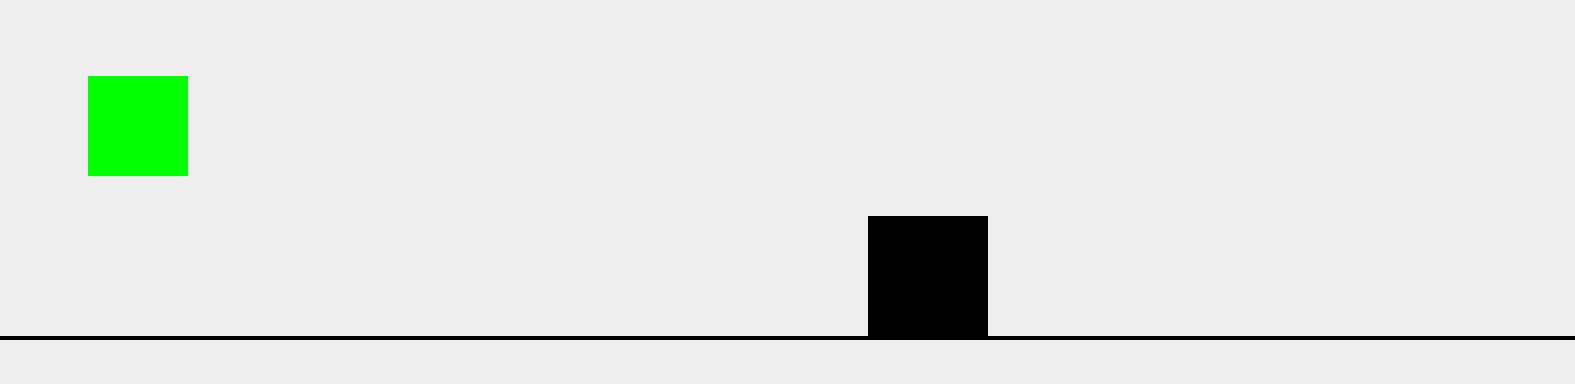
\includegraphics[width=0.5\textwidth]{images/jumpingDinoUmg.png}  \end{center}
    \caption{Jumping Dino Umgebung}
    \label{fig:2-Wege-2}
\end{figure}

Bei jedem Tick kann der Agent zwischen zwei Aktionen wählen, JUMP und NOTHING. Befindet sich der Agent bereits im Sprung, so ist es dennoch möglich die Aktion JUMP auszuwählen, sie hat jedoch keinen Effekt. Eine Episode endet, wenn eine Kollision zwischen dem Dino und dem Hindernis registriert wird.
\par 
Für die Untersuchungen wird zwischen zwei Szenarien unterschieden:
\par 
\textit{Simple}. Bei dieser Variante wandern die Hindernisse immer mit der gleichen Geschwindigkeit (30px pro Tick) nach links. Außerdem erscheinen sie immer im gleichen Abstand, d.h. erreicht die rechte Kante des Hindernisses den linken Bildschirmrand, so wird sofort ein neues Hindernis gespwant an der Position $x=860$. Es ergeben sich 31 mögliche Positionen, in der sich ein Hindernis in der Umwelt befinden kann ($x=860, x=830, \dots, x=-10, x=-40$).
\par 
\textit{Advanced}. Um die Umwelt anspruchsvoller zu gestalten, werden in diesem Szenario ein paar Änderungen vorgenommen. Statt einer festen Geschwindigkeit, bewegen sich die Hindernisse nun mit vier unterschiedlichen Geschwindigkeiten. Dies sorgt dafür, dass die Geschwindigkeit nun auch ein Faktor ist, der für einen Sprung des Dinos entscheidend ist. Bei sehr schnellen Hindernissen muss der Dino frühzeitig springen, um z.B. bei zwei aufeinanderfolgenden schnellen Hindernissen überhaupt in der Lage zu sein, das zweite Hindernis zu überspringen. Hingegeben muss er lernen, bei sehr langsamen Hindernissen erst sehr spät zu springen, um bei der Landung nicht zu kollidieren. Mit einer gleichen Wahrscheinlichkeit kann die Geschwindigkeit den Wert 10px, 21px, 48px oder 105px annehmen.
\par
Eine weitere Anpassung bei dem \textit{Jumping Dino Advanced} ist, dass die Hindernisse nicht immer mit dem gleichen Abstand spawnen, sondern ebenfalls zufällig mit vier unterschiedlichen Werten ($x=1630, x=1694, x=1718, x=1814$). Insgesamt ergeben sich 827 mögliche Positionen, die ein Hindernis einnehmen kann.

\subsubsection{Zustandsmodellierung}
Für eine korrekt gewählt Zustandsmodellierung, die genug aber nicht redundante Informationen beinhaltet, um die optimalen Entscheidung zu treffen, ist zunächst die Problemstellung genauer zu betrachten. 
\par 
In dem \textit{Jumping Dino Simple} Szenario muss der Agent lernen, im richtigen Moment die Aktion JUMPING durchzuführen. Anders ausgedrückt, kann der Agent in der Theorie immer die Aktion NOTHING wählen, muss aber bei einem bestimmten Abstand zu dem Hindernis die Aktion JUMP ausführen. Im Grunde ist dies eine Schwellwertsuche, bei der vorerst angenommen wird, dass alleine die Distanz zu dem Hindernis ausreichend ist, um das Problem zu lösen.
\par 
Den Zustand nur anhand der Distanz zu verwirklichen ist bei der \textit{Advanced} Variante nicht ausreichend, um optimale Entscheidung zu treffen. Schnelle Hindernisse müssen frühzeitiger übersprungen werden, langsame hingehen erst kurz vor einer Kollision. Eine zweite Information muss somit gegeben sein, die Geschwindigkeit der Hindernisse.
\par 
Im späteren Verlauf der Untersuchungen zu dem Konvergenzverhalten, die in Kapitel 5 näher erläutert werden, stellt sich heraus, dass der Zustand um eine boolische Flag erweitert werden muss, die aussagt, ob der Dino sich im Sprung befindet oder nicht. 
Es ergeben sich insgesamt drei unterschiedliche Zustandsmodellierungen, die auf folgenden Variablen beruhen:
\begin{itemize}
 \item $dist$: \textit{Integer}, Abstand zwischen rechter Kante des Dinos und  linker Kante des Hindernisses
 \item $inJump$: \textit{Boolean}, Boolischer Wert, ob sich der Dino in einem Sprung befindet und somit die Aktion \textit{JUMP} keine Auswirkung hat.
 \item $obsSpeed$: \textit{Integer}, Geschwindigkeit, mit der das Hindernis nach links wandert. Bei dem \textit{Jumping Dino Advanced} kann diese Variable vier unterschiedliche Werte annehmen.    
\end{itemize}
\begin{equation}
    Z_{1} =  \begin{bmatrix} dist\\   \end{bmatrix}, \quad
    Z_{2} =  \begin{bmatrix} dist \\ inJump   \end{bmatrix}, \quad
    Z_{3} =  \begin{bmatrix} dist \\ inJump \\ obsSpeed   \end{bmatrix}
\end{equation}

Die Kombination des Zustandraumes mit den zwei ausführbaren Aktionen ergibt die Anzahl der möglichen Zustands-Aktions-Paare, für die Werte in der Aktions-Nutzentabelle gespeichert werden. Es gibt zwei Szenarien \textit{Simple} und \textit{Advanced} und drei Zustandsmodellierungen $Z_1, Z_2$ und $Z_3$.
Für das Szenario \textit{Simple} ist die Modellierung $Z_3$ redundant, da die Variable $obsSpeed$ nur einen Wert annehmen kann. Wie bereits erwähnt, muss der $obsSpeed$ bei der \textit{Advanced} Variante gegegen sein. 
\par 
Wichtig zu erwähnen ist, dass diese Werte sich auf die tatsächlich möglichen $(s,a)$-Paare beziehen. D.h. für die \textit{Simple} Variante ergeben sich für $Z_2$ in der Theorie 62 mögliche Zustände (Abstand des Hindernisses * im Sprung oder nicht, $31*2$). Die Nutzentablle registriert jedoch nur 58 Zustände, da einige Zustände gar nicht erreicht werden können. Für die Abstände $-40, -10, 20$ und $50$ existieren nur die Kombinationen mit $inJump = true$. Der Dino musste vorher springen bzw. befindet sich im Sprung, da ansonsten die Episode zuvor bei einer Kollision vorzeitig beendet werden würde. Das erklärt die abweichenden Größen im Vergleich zu den Werten der theoretischen Kombinationen.
\par 
Gesamtanzahl aller gespeicherten Aktions-Nutzen:
\begin{equation}
G_{simple, Z_1} = 62, \quad
G_{simple, Z_2} = 116, \quad
G_{advanced, Z_3} = 4146 \quad 
\end{equation}


\subsubsection{Belohnungsfunktion}
Im Kapitel \ref{sec:belohnung} wurde darauf eingegangen, wie in eine Belohnungsfunktion gewählt werden sollte. Die Schlussfolgerung war, dass eine Belohnungsfunktion dem Agenten vermitteln soll, \textit{was} er erreichen soll und nicht \textit{wie} er es erreichen soll \cite[S.~54]{Sutton1998}.
\par 
Die Aufgabe des hüpfenden Dinos besteht darin, die Episode so lang wie möglich zu überleben. Anders formuliert soll die Episode eine maximale Anzahl von Zeitstempeln andauern. Um dieses Ziel als Belohungssignal zu modellieren, reicht es aus dem Agenten zu jedem Zeitpunkt $t$ eine Belohnung von +1 mitzuteilen. Einzige Ausnahme ist hierbei das Erreichen eines Terminalzustandes. Kollidiert der Dino mit einem Hindernis, so erhält er die Belohnung +0 und die Episode ist beendet. Der Gewinn einer Episode richtet sich somit nach der Anzahl der Zeitstempel. Eine explizite Modellierung der Hindernisse oder die Vergabe von Belohnungen für das Überspringen dieser ist nicht notwendig, da der Agent implizit lernt, Hindernisse zu überspringen, um die Summe der Belohnungen zu maximieren. 
\par 
//TODO
\par 

	\subsection{Ant-Game}
	\subsubsection{Problemstellung}
		\subsubsection{Zustandsmodellierung}
	\subsection{Ergebnisse}
\section{Fazit}
\section{Ausblick}

\pagebreak
\bibliography{quellen}
\pagebreak

Bellman Optimality Equation:
\begin{equation}\label{eq:bellman}
    \begin{aligned}
    q_*(s,a) &= \EX [R_{t+1} + \gamma \max_{a'}q_*(S_{t+1}, a') \mid S_t = s, A_t = a] \\
    &= \sum_{s',r}p(s', r\mid s, a)[r + \gamma \max_{a'}q_*(s', a')]
    \end{aligned}
\end{equation}
\end{document}
